\documentclass[aspectratio=169]{beamer}
\usetheme{Madrid}
\usecolortheme{whale}
\setbeamertemplate{navigation symbols}{}

% Paquetes necesarios
\usepackage[utf8]{inputenc}
\usepackage[spanish]{babel}
\usepackage{graphicx}
\usepackage{tikz}
\usepackage{booktabs}
\usepackage{colortbl}
\usepackage{xcolor}
\usepackage{multirow}
\usepackage{listings}

% Configuración de listings para Beamer
\lstset{
    basicstyle=\tiny\ttfamily,
    breaklines=true,
    frame=single,
    numbers=left,
    numberstyle=\tiny,
    showstringspaces=false,
    tabsize=2,
    captionpos=b,
    literate={á}{{\'a}}1 {é}{{\'e}}1 {í}{{\'i}}1 {ó}{{\'o}}1 {ú}{{\'u}}1 {ñ}{{\~n}}1 {¿}{{?`}}1 {¡}{{!`}}1
}

% Colores personalizados
\definecolor{uaiBlue}{RGB}{0,84,147}
\definecolor{uaiOrange}{RGB}{255,102,0}
\definecolor{lightBlue}{RGB}{173,216,230}
\definecolor{lightOrange}{RGB}{255,218,185}

% Configuración del tema
\setbeamercolor{title}{fg=white,bg=uaiBlue}
\setbeamercolor{frametitle}{fg=uaiBlue,bg=lightBlue}
\setbeamercolor{section title}{fg=white,bg=uaiOrange}

% Configuración de fuentes más pequeñas
\setbeamerfont{frametitle}{size=\small}
\setbeamerfont{block title}{size=\footnotesize}
\setbeamerfont{block body}{size=\scriptsize}

\title{\footnotesize \textbf{Nivelación en Redes}}
\subtitle{\footnotesize TICS413 - Seguridad TI}
\author{\footnotesize Profesores del Curso}
\institute{\footnotesize UAI}
\date{\footnotesize \today}

\begin{document}

% Portada
\begin{frame}
\maketitle
\end{frame}

% Índice
\begin{frame}
\frametitle{Contenido de la Sesión}
\begin{columns}
\column{0.5\textwidth}
\begin{block}{Fundamentos de Redes}
\begin{itemize}
\item ¿Qué es una Red?
\item Evolución de las Redes
\item Conceptos Básicos de Paquetes
\item Estructura de Paquetes IP
\item Conmutación de Paquetes vs. Circuitos
\item Segmentación de Redes
\end{itemize}
\end{block}

\begin{block}{Arquitectura de Protocolos}
\begin{itemize}
\item Pila TCP/IP
\item Modelo OSI
\item Encapsulación y Desencapsulación
\end{itemize}
\end{block}

\column{0.5\textwidth}
\begin{block}{Capas del Modelo OSI}
\begin{itemize}
\item Capas 1-4: Física a Transporte
\item Capas 5-7: Sesión a Aplicación
\item Funcionamiento de las Capas
\end{itemize}
\end{block}

\begin{block}{Conceptos Avanzados}
\begin{itemize}
\item Servicios de Red (Puertos)
\item Análisis de Paquetes
\end{itemize}
\end{block}
\end{columns}

\begin{block}{Conexión con la Seguridad}
\textbf{Estos conceptos son la base para entender la seguridad en redes.} 
Cada capa del modelo OSI presenta vulnerabilidades específicas que los 
profesionales de seguridad deben conocer y proteger.
\end{block}
\end{frame}

% ========================================
% SLIDE 1: ¿Qué es una red?
% ========================================
\section{¿Qué es una Red?}

\begin{frame}
\frametitle{¿Qué es una Red?}
\begin{block}<7->{Concepto Clave}
  Una red no es solo cables y dispositivos, sino un \textbf{sistema organizado} 
donde cada elemento tiene una función específica en la comunicación de datos.
  \end{block}
\begin{itemize}
\item<1-> \textbf{Definición}: Sistema que permite la comunicación entre dispositivos
\item<2-> \textbf{Analogía}: Como las calles que conectan casas en una ciudad
\item<3-> \textbf{Objetivo}: Compartir recursos e información de manera eficiente
\end{itemize}
\end{frame}

\begin{frame}
  \frametitle{¿Qué es una Red?}
  \begin{center}
  \Large \textbf{Una red es como un sistema de carreteras para la información}
  \end{center}
  
  \begin{center}
  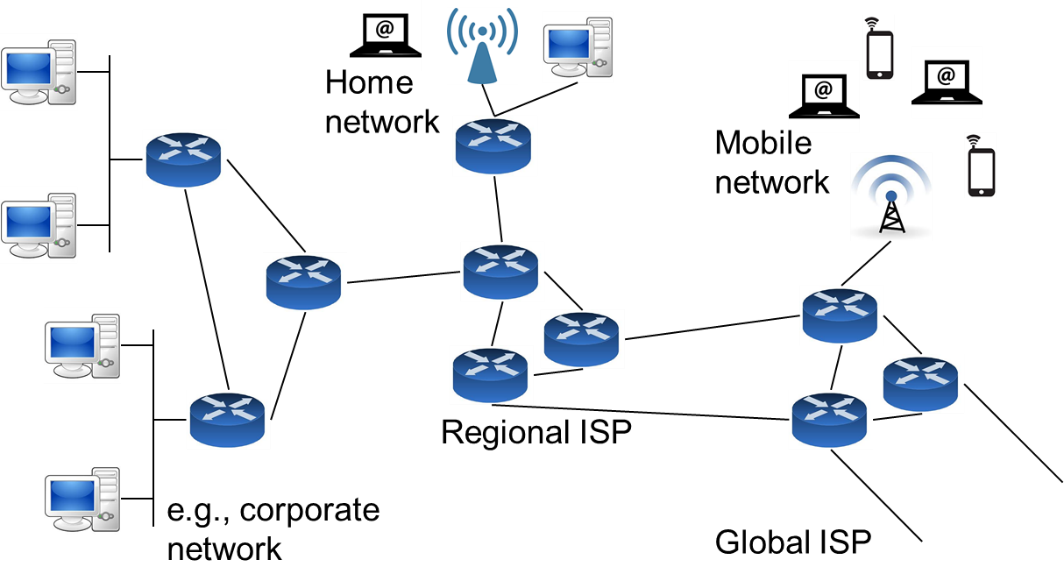
\includegraphics[width=0.5\textwidth]{figuras/image100.png}
  \small \textit{Concepto básico de redes de comunicación}
  \end{center}
  \end{frame}

\begin{frame}
  \frametitle{Tipos de Redes}

\begin{itemize}
\item \textbf{WAN} (Wide Area Network): Más de 10 km - Como las autopistas entre ciudades
\item \textbf{LAN} (Local Area Network): Menos de 10 km - Como las calles de un barrio
\item \textbf{PAN} (Personal Area Network): 10-20 m - Como la conexión Bluetooth de tu celular
\end{itemize}

\end{frame}

% ========================================
% SLIDE: Evolución de las Redes
% ========================================
\begin{frame}
\frametitle{Evolución de las Redes}

\begin{center}
\Large \textbf{De los telégrafos a Internet: evolución de la comunicación}
\end{center}

\begin{columns}
\column{0.5\textwidth}
\begin{block}<1->{Redes de Telégrafo (1800s)}
\begin{itemize}
\item<1-> \textbf{Código Morse}: Secuencias de puntos y rayas
\item<2-> \textbf{Store-and-forward}: Almacenamiento y reenvío
\item<3-> \textbf{Message Switching}: Mensajes completos se enrutan
\item<4-> \textbf{Sin circuito dedicado}: Recursos compartidos
\end{itemize}
\end{block}

\begin{block}<5->{Redes Telefónicas (1900s)}
\begin{itemize}
\item<5-> \textbf{Circuit Switching}: Recursos dedicados por llamada
\item<6-> \textbf{Multiplexing}: T1 (24 señales de voz digitalizadas)
\item<7-> \textbf{Connection-oriented}: Configuración de sesión previa
\item<8-> \textbf{Ruta fija}: Mismo camino para todos los datos
\end{itemize}
\end{block}

\column{0.5\textwidth}
\begin{block}<9->{Internet y Redes de Computadoras (1960s+)}
\begin{itemize}
\item<9-> \textbf{Packet Switching}: Datos divididos en paquetes
\item<10-> \textbf{Statistical Multiplexing}: Recursos compartidos dinámicamente
\item<11-> \textbf{Store-and-forward}: Cada router almacena y reenvía
\item<12-> \textbf{IP Protocol}: Servicio de datagramas global
\end{itemize}
\end{block}

\begin{block}<13->{Ventajas del Packet Switching}
\begin{itemize}
\item<13-> \textbf{Mejor para datos bursty}: Uso eficiente de ancho de banda
\item<14-> \textbf{Recursos compartidos}: Más usuarios pueden usar la red
\item<15-> \textbf{Sin configuración}: No requiere setup de llamada
\item<16-> \textbf{Escalabilidad}: Soporta más usuarios simultáneos
\end{itemize}
\end{block}
\end{columns}
\end{frame}

% ========================================
% SLIDE: ¿Qué es una Red?
% ========================================
\begin{frame}
\frametitle{Elementos fundamentales de una red de computadoras}

\begin{center}
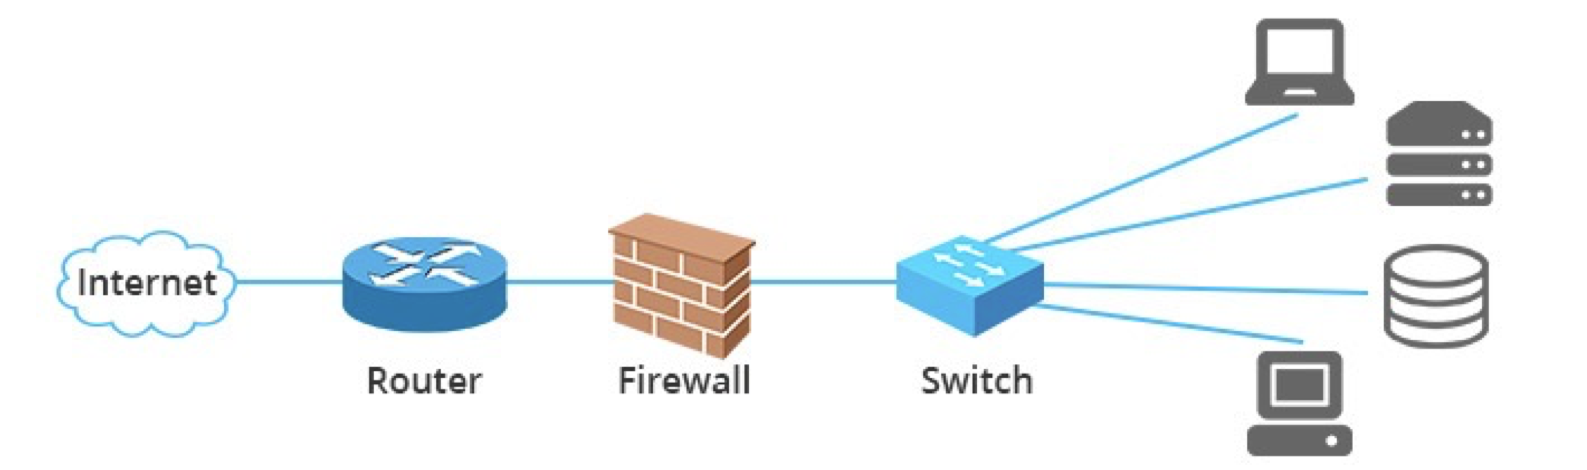
\includegraphics[width=0.8\textwidth]{figuras/image1001.png}
\end{center}

\begin{block}<2->{Componentes de una Red}
\begin{itemize}
\item<2-> \textbf{Internet}: Red externa que conecta con el mundo
\item<3-> \textbf{Router}: Dispositivo que dirige el tráfico entre redes
\item<4-> \textbf{Firewall}: Barrera de seguridad que filtra el tráfico
\item<5-> \textbf{Switch}: Conecta múltiples dispositivos en la misma red local
\item<6-> \textbf{Dispositivos finales}: Laptops, servidores, bases de datos
\end{itemize}
\end{block}
\end{frame}

% ========================================
% SLIDE 3-4: Network Organization & Connectivity
% ========================================
\begin{frame}
\frametitle{Organización de Redes y Conectividad}

\begin{center}
\Large \textbf{¿Por qué las redes punto a punto no escalan?}
\end{center}

\begin{block}<1->{Problema de Escalabilidad}
\begin{itemize}
\item<1-> \textbf{Complejidad O(N²)}: El número de enlaces crece cuadráticamente
\item<2-> \textbf{Agregar un nodo}: Requiere enlaces a todos los nodos existentes
\item<3-> \textbf{Costo de mantenimiento}: Cada enlace adicional aumenta la complejidad
\item<4-> \textbf{Administración}: Difícil gestionar tantas conexiones
\end{itemize}
\end{block}

\begin{block}<5->{Ejemplo Numérico}
\begin{itemize}
\item<5-> \textbf{5 nodos}: 10 enlaces
\item<6-> \textbf{10 nodos}: 45 enlaces  
\item<7-> \textbf{100 nodos}: 4,950 enlaces
\item<8-> \textbf{1000 nodos}: 499,500 enlaces
\end{itemize}
\end{block}
\end{frame}
  
% ========================================
% SLIDE 5: Network Structure
% ========================================
\begin{frame}
\frametitle{Estructura de Redes}

\begin{center}
\Large \textbf{Necesidad de compartir infraestructura}
\end{center}

\begin{block}<1->{Ventajas de la Estructura Jerárquica}
\begin{itemize}
\item<1-> \textbf{Compartir infraestructura}: Múltiples redes usan los mismos routers
\item<2-> \textbf{Routers y switches}: Dispositivos especializados para cada función
\item<3-> \textbf{Reducir costos}: No duplicar equipos para cada red
\item<4-> \textbf{Mejor escalabilidad}: Agregar redes sin afectar las existentes
\end{itemize}
\end{block}

\begin{block}<5->{Componentes Clave}
\begin{itemize}
\item<5-> \textbf{Switches}: Conectan dispositivos en la misma red local
\item<6-> \textbf{Routers}: Conectan diferentes redes y subredes
\item<7-> \textbf{ISP Regional}: Proporciona conectividad a múltiples clientes
\item<8-> \textbf{ISP Global}: Backbone de Internet
\end{itemize}
\end{block}
\end{frame}

% ========================================
% SLIDE 7: Usage Models
% ========================================
\begin{frame}
\frametitle{Modelos de Uso de Redes}

\begin{center}
\Large \textbf{Cliente/Servidor vs Peer-to-Peer}
\end{center}

\begin{block}{Ventajas y Desventajas}
\begin{itemize}
\item \textbf{Estrella}: Fácil mantenimiento, punto único de falla
\item \textbf{Anillo}: Eficiente, pero si se rompe un enlace se pierde la red
\item \textbf{Malla}: Muy confiable, pero costosa de implementar
\item \textbf{Árbol}: Escalable, pero dependiente del nodo raíz
\end{itemize}
\end{block}
\end{frame}

% ========================================
% SLIDE 8: Packet Switched Routers
% ========================================
\begin{frame}
\frametitle{Routers con Conmutación de Paquetes}

\begin{center}
\Large \textbf{Multiplexación y demultiplexación en routers}
\end{center}

\begin{center}
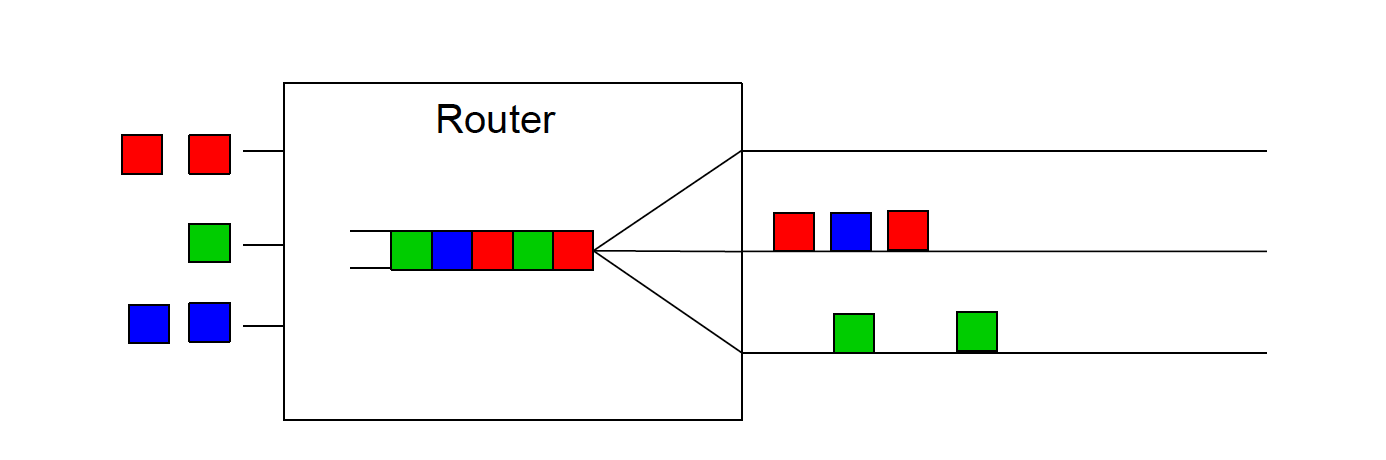
\includegraphics[width=0.8\textwidth]{figuras/router.png}
\end{center}

\begin{block}<1->{Proceso de Conmutación}
\begin{itemize}
\item<1-> \textbf{Multiplexación}: Paquetes de múltiples entradas se combinan
\item<2-> \textbf{Cola interna}: Paquetes esperan en buffer FIFO
\item<3-> \textbf{Demultiplexación}: Basada en encabezados se envían a salidas
\item<4-> \textbf{Enrutamiento}: Cada paquete toma su ruta específica
\end{itemize}
\end{block}

\begin{block}{Ventajas del Packet Switching}
\begin{itemize}
\item<1-> \textbf{Eficiencia}: Mejor uso del ancho de banda
\item<2-> \textbf{Flexibilidad}: Rutas dinámicas según congestión
\item<3-> \textbf{Escalabilidad}: Soporta más usuarios simultáneos
\item<4-> \textbf{Recuperación}: Reruteo automático en caso de fallas
\end{itemize}
\end{block}
\end{frame}

% ========================================
% SLIDE 9: Managing Complexity
% ========================================
\begin{frame}
\frametitle{Gestionando la Complejidad}

\begin{center}
\Large \textbf{Problemas de escala y variedad tecnológica}
\end{center}

\begin{block}<1->{Problemas de Escala}
\begin{itemize}
\item<1-> \textbf{Complejidad O(N²)}: Las redes punto a punto no escalan
\item<2-> \textbf{Administración}: Difícil gestionar muchas conexiones
\item<3-> \textbf{Costos}: Cada enlace adicional es costoso
\item<4-> \textbf{Mantenimiento}: Fallas afectan toda la red
\end{itemize}
\end{block}

\begin{block}<5->{Variedad Tecnológica}
\begin{itemize}
\item<5-> \textbf{Medios físicos}: Cable, fibra, Wi-Fi, móvil
\item<6-> \textbf{Protocolos}: Diferentes estándares y versiones
\item<7-> \textbf{Dispositivos}: Múltiples fabricantes y modelos
\item<8-> \textbf{Requerimientos}: Diferentes necesidades de calidad de servicio
\end{itemize}
\end{block}
\end{frame}

\begin{frame}
\frametitle{Gestionando la Complejidad}

\begin{center}
\Large \textbf{¿Cómo resolver los problemas de escala y variedad tecnológica?}
\end{center}

\begin{block}{Solución: Arquitectura en Capas}
\begin{itemize}
\item<1-> \textbf{Separación de responsabilidades}: Cada capa tiene una función específica
\item<2-> \textbf{Independencia}: Las capas pueden evolucionar por separado
\item<3-> \textbf{Interoperabilidad}: Diferentes implementaciones pueden comunicarse
\item<4-> \textbf{Modularidad}: Fácil agregar o modificar funcionalidades
\end{itemize}
\end{block}
\end{frame}

% ========================================
% SLIDE 10-12: Networking Layers & Layering
% ========================================
\begin{frame}
\frametitle{Capas de Redes y Principios de Diseño}

\begin{center}
\Large \textbf{Introducción al modelo de capas}
\end{center}

\begin{center}
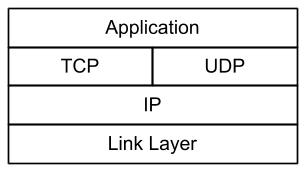
\includegraphics[width=0.35\textwidth]{figuras/tcpsobreip.png}
\end{center}

\begin{block}<1->{Principios de Diseño}
\begin{itemize}
\item<1-> \textbf{Separación de preocupaciones}: Cada capa tiene responsabilidades únicas
\item<2-> \textbf{Encapsulación}: Cada capa agrega su encabezado específico
\item<3-> \textbf{Independencia}: Las capas superiores no dependen de las inferiores
\item<4-> \textbf{Interfaz bien definida}: Comunicación estándar entre capas
\end{itemize}
\end{block}

\end{frame}


\begin{frame}
\frametitle{Capas de Redes y Principios de Diseño}

\begin{center}
\Large \textbf{Introducción al modelo de capas}
\end{center}

\begin{center}
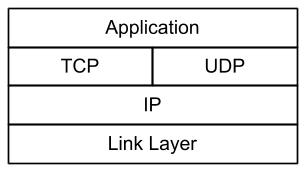
\includegraphics[width=0.35\textwidth]{figuras/tcpsobreip.png}
\end{center}

\begin{block}{Beneficios del Modelo}
\begin{itemize}
\item<1-> \textbf{Modularidad}: Fácil desarrollo y mantenimiento
\item<2-> \textbf{Reutilización}: Implementaciones pueden reutilizarse
\item<3-> \textbf{Estándares}: Protocolos bien definidos por capa
\item<4-> \textbf{Educativo}: Facilita la comprensión de redes
\end{itemize}
\end{block}
\end{frame}

% ========================================
% SLIDE 14-15: OSI vs TCP/IP
% ========================================
\begin{frame}
\frametitle{OSI vs TCP/IP - Comparación}

\begin{center}
\Large \textbf{¿Por qué dos modelos de referencia?}
\end{center}

\begin{columns}
\column{0.5\textwidth}
\begin{block}{Modelo OSI (7 Capas)}
\begin{itemize}
\item \textbf{Capa 7}: Aplicación (HTTP, FTP, DNS)
\item \textbf{Capa 6}: Presentación (SSL/TLS, JPEG)
\item \textbf{Capa 5}: Sesión (RPC, NetBIOS)
\item \textbf{Capa 4}: Transporte (TCP, UDP)
\item \textbf{Capa 3}: Red (IP, ICMP)
\item \textbf{Capa 2}: Enlace (Ethernet, ARP)
\item \textbf{Capa 1}: Física (Cable, Wi-Fi)
\end{itemize}
\end{block}
      
\column{0.5\textwidth}
\begin{block}{Modelo TCP/IP (4 Capas)}
\begin{itemize}
\item \textbf{Aplicación}: HTTP, FTP, DNS, SMTP
\item \textbf{Transporte}: TCP, UDP
\item \textbf{Internet}: IP, ICMP
\item \textbf{Acceso a Red}: Ethernet, Wi-Fi
\end{itemize}
\end{block}
\end{columns}
\end{frame}

\begin{frame}
\frametitle{OSI vs TCP/IP - Comparación}

\begin{center}
\Large \textbf{¿Por qué dos modelos de referencia?}
\end{center}

\begin{center}
\begin{table}
\centering
\begin{tabular}{|c|c|c|}
\hline
\textbf{OSI (7 capas)} & \textbf{TCP/IP (4 capas)} & \textbf{Protocolo} \\
\hline
\rowcolor{lightBlue} Aplicación (7) & \multirow{3}{*}{Aplicación} & HTTP, FTP, DNS \\
\rowcolor{lightBlue} Presentación (6) & & SSL/TLS \\
\rowcolor{lightBlue} Sesión (5) & & RPC \\
\rowcolor{lightOrange} Transporte (4) & Transporte & TCP, UDP \\
\rowcolor{lightBlue} Red (3) & Internet & IP, ICMP \\
\rowcolor{lightOrange} Enlace (2) & \multirow{2}{*}{Acceso a red} & Ethernet, ARP \\
\rowcolor{lightOrange} Física (1) & & Wi-Fi, cable \\
\hline
\end{tabular}
\end{table}
\end{center}

\begin{block}{¿Por qué TCP/IP es más usado?}
\textbf{TCP/IP es el estándar de facto en Internet} porque es más simple, 
práctico y fue desarrollado específicamente para resolver problemas reales 
de comunicación. El modelo OSI, aunque más completo teóricamente, es 
demasiado complejo para implementaciones prácticas.
\end{block}
\end{frame}

% ========================================
% SLIDE: Segmentación de Redes
% ========================================
\begin{frame}
\frametitle{Segmentación de Redes}

\begin{center}
\Large \textbf{División de redes en subredes más pequeñas}
\end{center}

\begin{center}
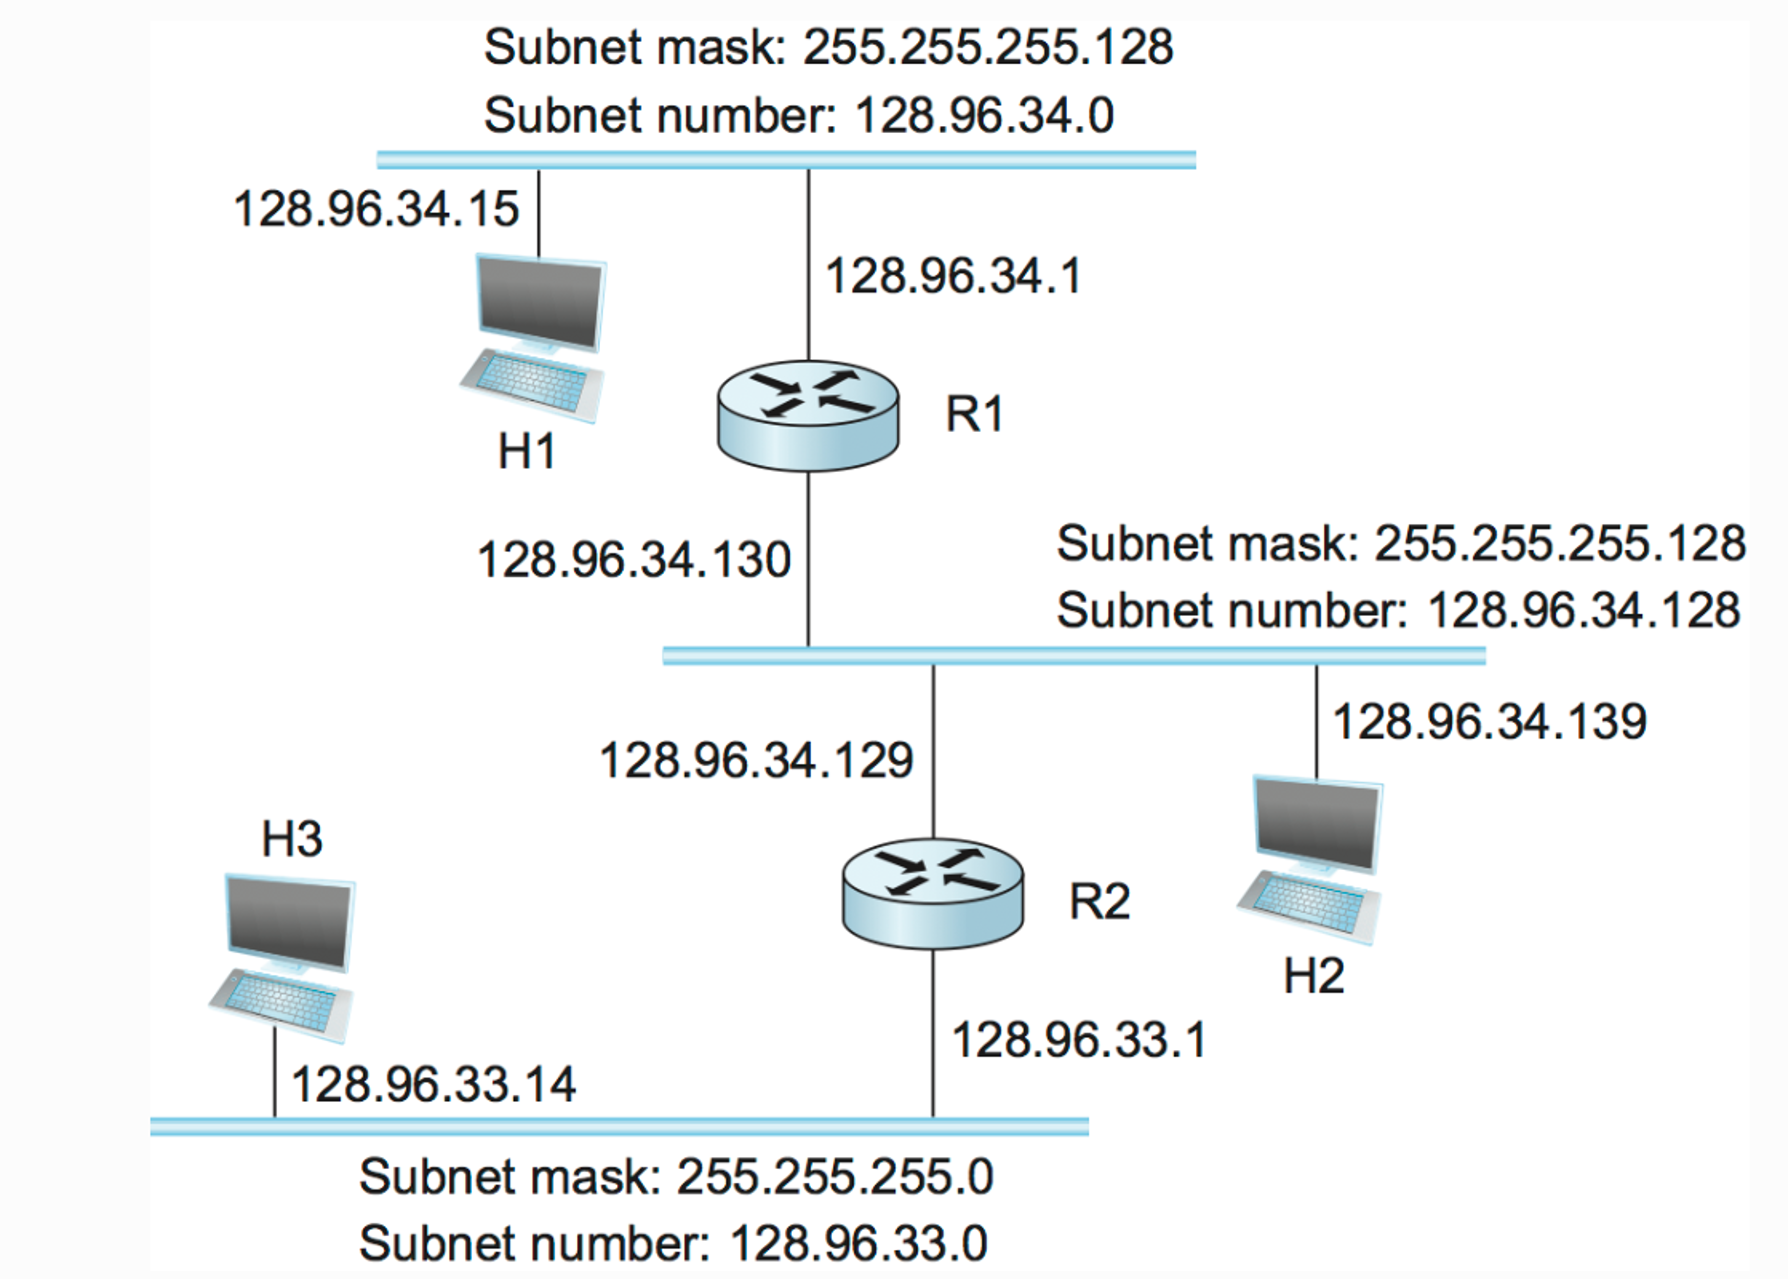
\includegraphics[width=0.5\textwidth]{figuras/image7.png}
\end{center}

\begin{block}<1->{¿Qué es el Subnetting?}
\begin{itemize}
\item<1-> \textbf{División lógica} de una red IP en subredes más pequeñas
\item<2-> \textbf{Máscaras de subred}: Definen el tamaño de cada subred
\item<3-> \textbf{Enrutamiento}: Los routers conectan diferentes subredes
\end{itemize}
\end{block}
\end{frame}

\begin{frame}
\frametitle{Segmentación de Redes}

\begin{center}
            \Large \textbf{División de redes en subredes más pequeñas}
            \end{center}
        
            
        \begin{block}<1->{Ejemplo de la Imagen}
        \begin{itemize}
        \item<2-> \textbf{Subred Superior}: 128.96.34.0/25 (máscara 255.255.255.128)
        \item<3-> \textbf{Subred Central}: 128.96.34.128/25 (máscara 255.255.255.128)
        \item<4-> \textbf{Subred Inferior}: 128.96.33.0/24 (máscara 255.255.255.0)
        \end{itemize}
        \end{block}
        \end{frame}

      % ========================================
      % SLIDE: Estructura de un Paquete IP
      % ========================================
      
      \begin{frame}
          \frametitle{Conceptos Básicos de Redes}
          \begin{center}
              \Large \textbf{Paquete}
              \end{center}
      \begin{block}<1->{¿Qué es un Paquete?}
      \begin{itemize}
      \item<1-> \textbf{Unidad básica de datos} que se transmite a través de una red
      \item<2-> Como un sobre de correo: tiene dirección de origen, destino y datos
      \item<3-> Se divide en \textbf{encabezado} (control) y \textbf{cuerpo} (datos)
      \end{itemize}
      \end{block}
      
      \begin{block}<4->{Direccionamiento Fundamental}
      \begin{itemize}
      \item<4-> \textbf{Dirección IP}: Identificador lógico de red (32 bits en IPv4)
      \item<5-> \textbf{Dirección MAC}: Identificador físico único del dispositivo
      \item<6-> \textbf{Conversiones}: Decimal, binario y hexadecimal para IPs
      \end{itemize}
      \end{block}
      \end{frame}
      
      % \begin{frame}
      % \frametitle{Estructura de un Paquete IP}
      % 
      % \begin{center}
      % \Large \textbf{Encabezado IPv4 detallado}
      % \end{center}
      % 
      % \begin{center}
      % 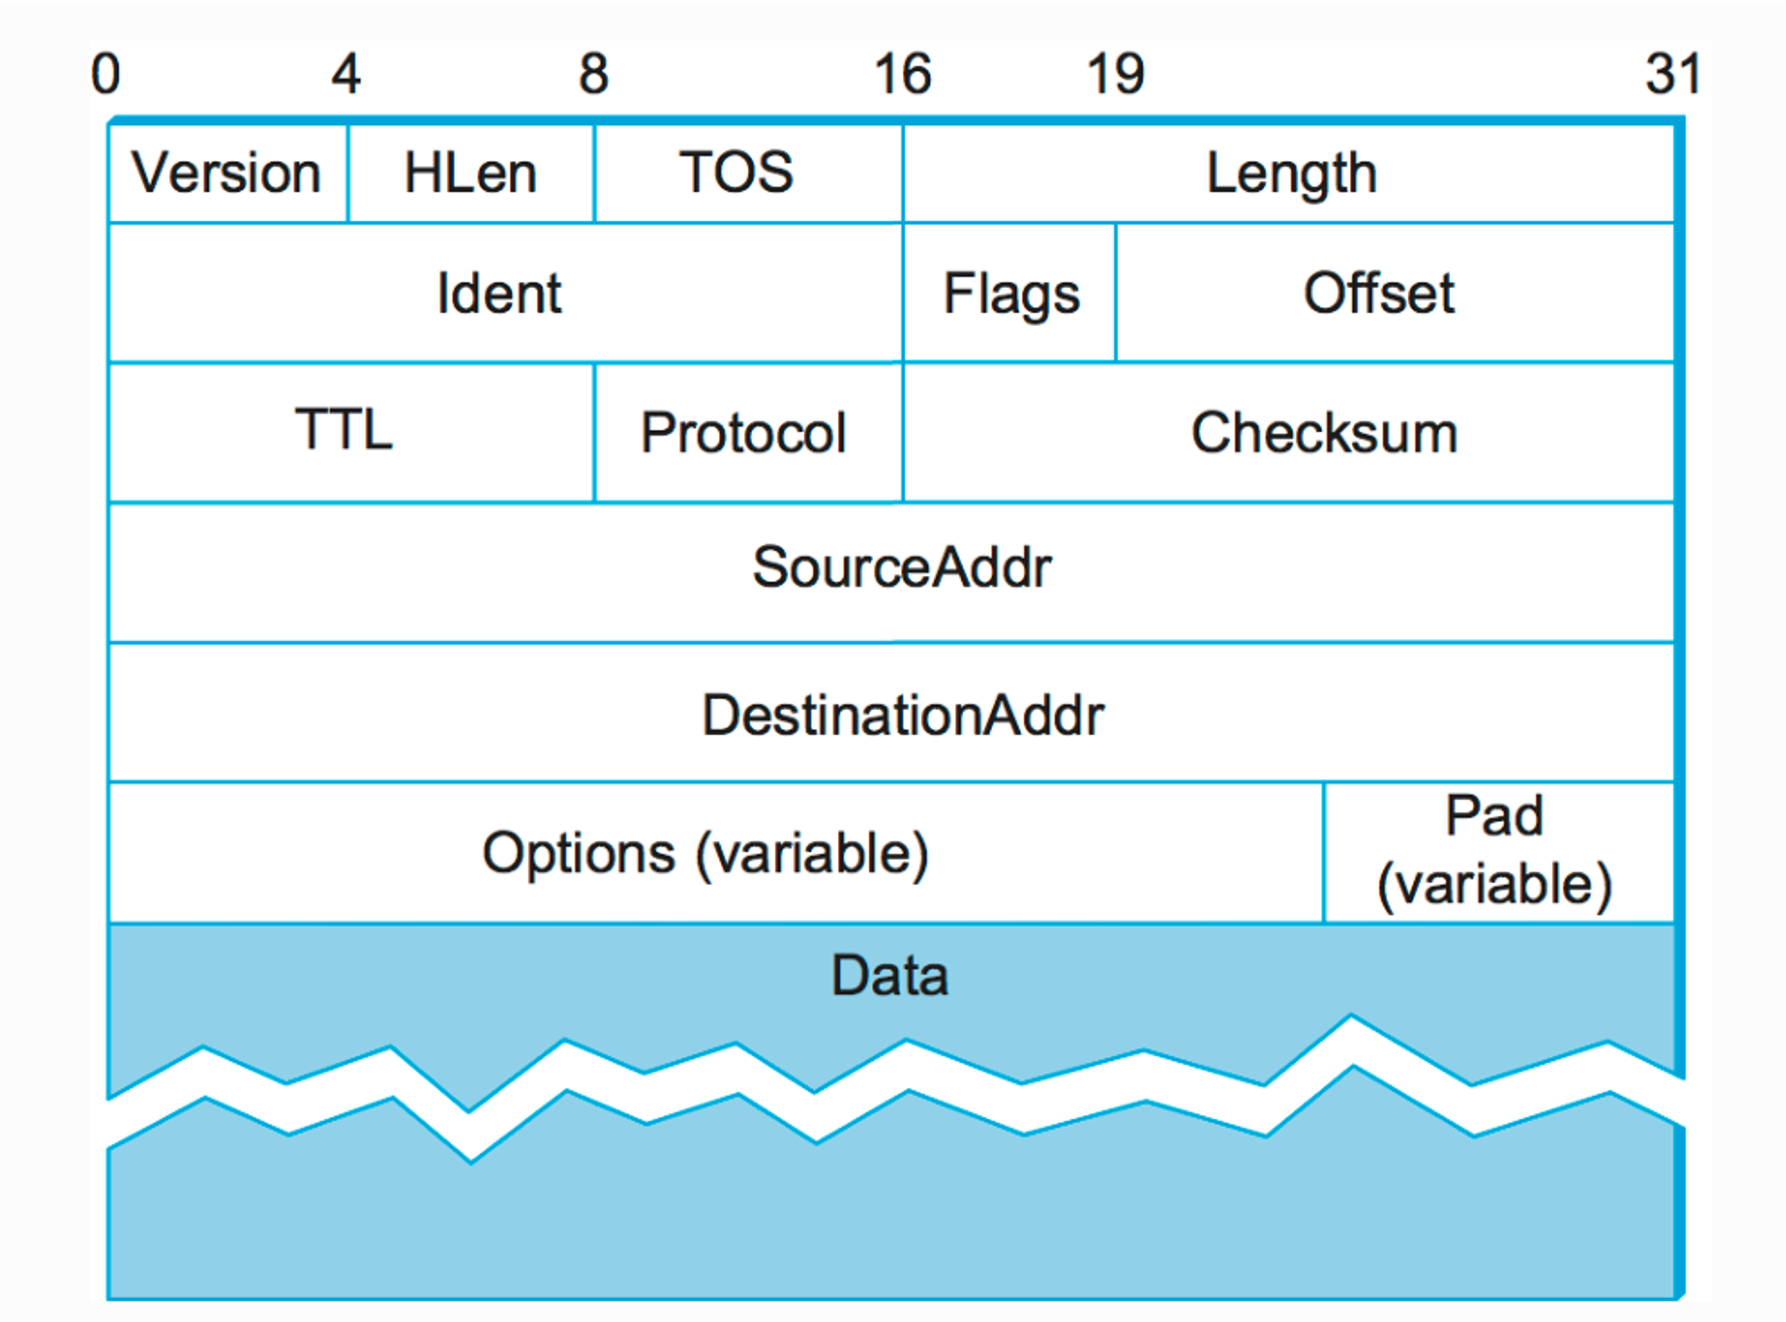
\includegraphics[width=0.8\textwidth]{figuras/image6.png}
      % \end{center}
      % \end{frame}
      \begin{frame}
      \frametitle{Estructura de un Paquete IP}
      \begin{block}<1->{Campos del Encabezado IPv4}
      \begin{itemize}
      \item<1-> \textbf{Version (4 bits)}: Versión del protocolo IP (IPv4 = 4)
      \item<2-> \textbf{HLen (4 bits)}: Longitud del encabezado en palabras de 32 bits
      \item<3-> \textbf{TOS (8 bits)}: Tipo de servicio para calidad de servicio
      \item<4-> \textbf{Total Length (16 bits)}: Longitud total del paquete
      \end{itemize}
      \end{block}
      
      \begin{block}<5->{Información de Control}
      \begin{itemize}
      \item<5-> \textbf{TTL (8 bits)}: Tiempo de vida del paquete
      \item<6-> \textbf{Protocol (8 bits)}: Protocolo de la capa superior (TCP/UDP)
      \item<7-> \textbf{Checksum (16 bits)}: Verificación de integridad del encabezado
      \end{itemize}
      \end{block}
      \end{frame}
      
      % ========================================
      % SLIDE: Conmutación de Paquetes vs. Circuitos
      % ========================================
      \begin{frame}
      \frametitle{Conmutación de Paquetes vs. Circuitos}
      
      \begin{center}
      \Large \textbf{¿Cómo se transfieren los datos a través de la red?}
      \end{center}
      
      \begin{columns}
      \column{0.5\textwidth}
      \begin{block}<1->{Circuit Switching (Redes Telefónicas)}
      \begin{itemize}
      \item<1-> \textbf{Recursos dedicados}: Ancho de banda reservado por llamada
      \item<2-> \textbf{Setup requerido}: Configuración de circuito antes de transmitir
      \item<3-> \textbf{Ruta fija}: Mismo camino para todos los datos
      \item<4-> \textbf{Rendimiento garantizado}: Sin retrasos de cola
      \item<5-> \textbf{Ineficiencia}: Recursos ociosos si no se usan
      \end{itemize}
      \end{block}
      
      \column{0.5\textwidth}
      \begin{block}<6->{Packet Switching (Internet)}
      \begin{itemize}
      \item<6-> \textbf{Recursos compartidos}: Ancho de banda usado según necesidad
      \item<7-> \textbf{Sin setup}: Los paquetes se envían inmediatamente
      \item<8-> \textbf{Rutas dinámicas}: Cada paquete puede tomar camino diferente
      \item<9-> \textbf{Retrasos variables}: Dependiendo de la congestión
      \item<10-> \textbf{Eficiencia}: Mejor uso del ancho de banda
      \end{itemize}
      \end{block}
      \end{columns}
      \end{frame}
      
      % ========================================
      % SLIDE: Pila de Protocolos TCP/IP
      % ========================================
      \begin{frame}
      \frametitle{Pila de Protocolos TCP/IP}
      
      \begin{center}
      \Large \textbf{Arquitectura de capas del conjunto de protocolos}
      \end{center}
      
      \begin{center}
      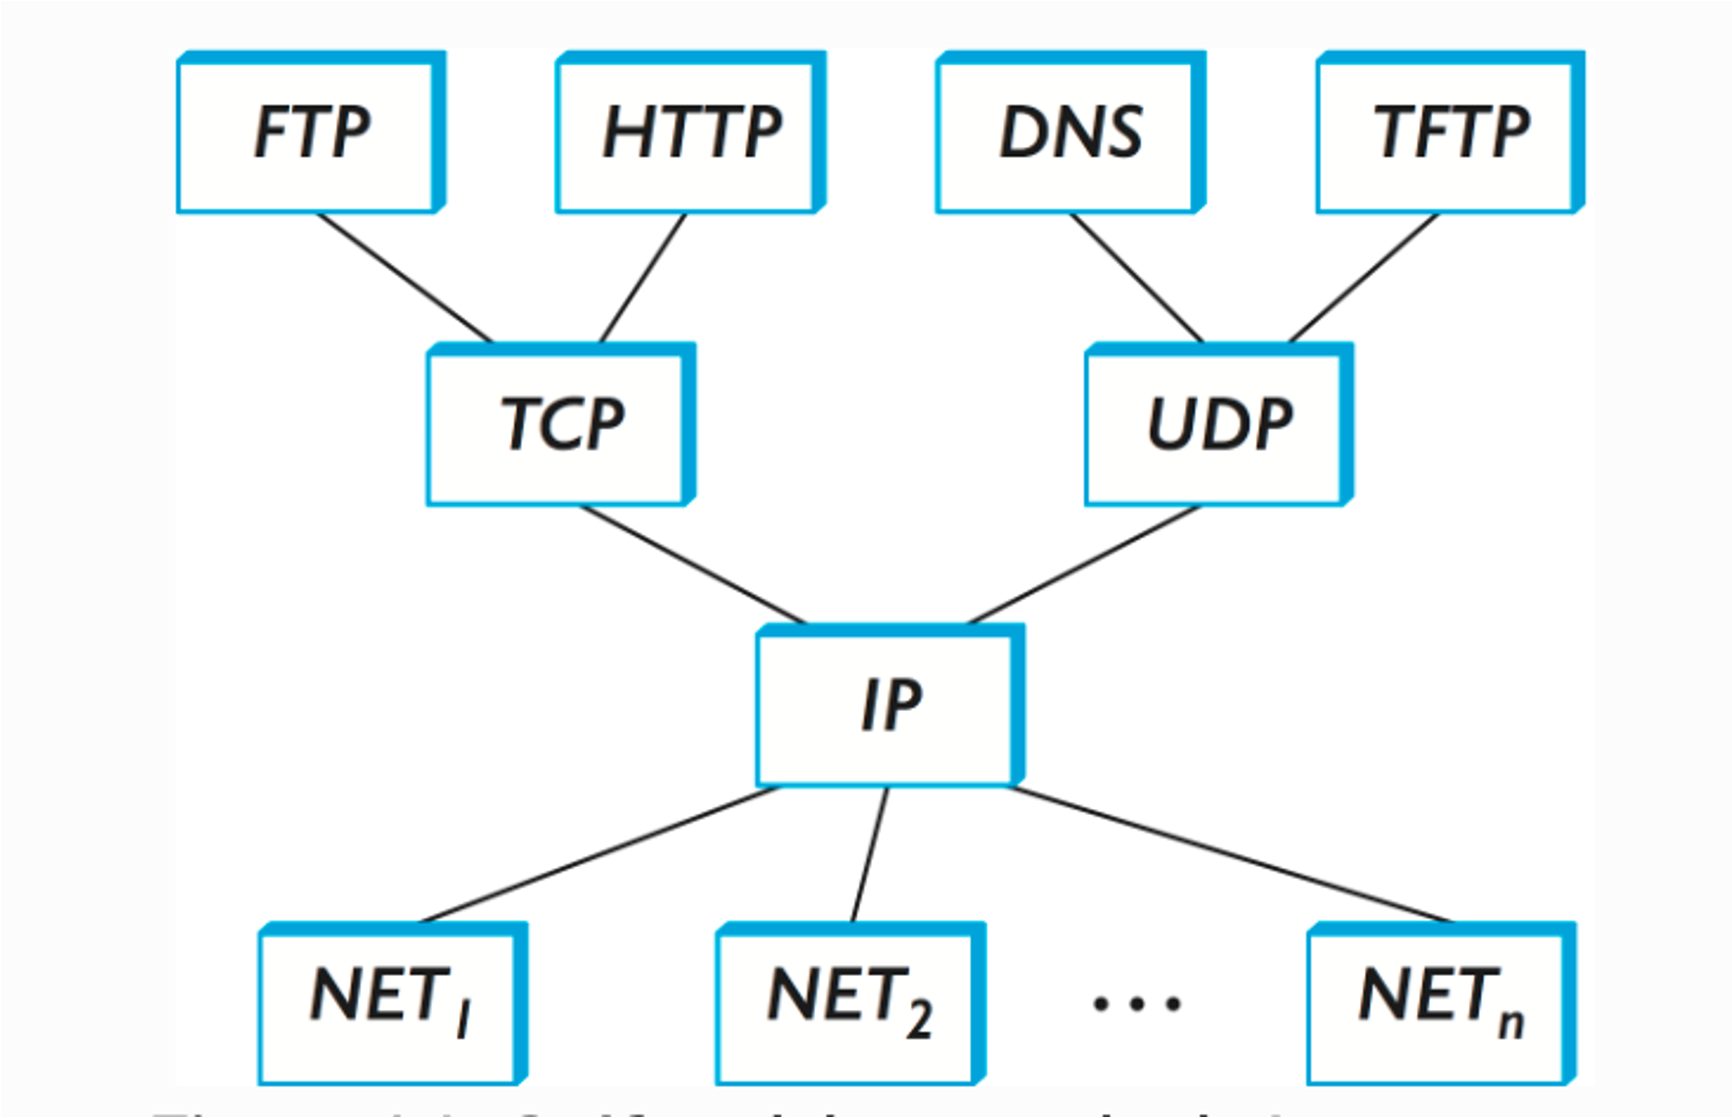
\includegraphics[width=0.4\textwidth]{figuras/image8.png}
      \end{center}
      \end{frame}
      
      \begin{frame}
          \frametitle{Pila de Protocolos TCP/IP}
      
      \begin{block}<1->{Capas del Modelo TCP/IP}
      \begin{itemize}
      \item<1-> \textbf{Capa de Aplicación}: FTP, HTTP, DNS, TFTP
      \item<2-> \textbf{Capa de Transporte}: TCP (confiable) y UDP (rápido)
      \item<3-> \textbf{Capa de Internet}: IP para enrutamiento
      \item<4-> \textbf{Capa de Acceso a Red}: Múltiples tecnologías de red
      \end{itemize}
      \end{block}
      
      \begin{block}<5->{Comunicación entre Capas}
      \begin{itemize}
      \item<5-> \textbf{Encapsulación}: Cada capa agrega su encabezado
      \item<6-> \textbf{Desencapsulación}: Cada capa remueve su encabezado
      \item<7-> \textbf{Independencia}: Las capas superiores no dependen de las inferiores
      \end{itemize}
      \end{block}
      \end{frame}
      
      % ========================================
      % SLIDE 16: Layer 1 & 2
      % ========================================
      \begin{frame}
      \frametitle{Capa 1 \& 2: Física y Enlace}
      
      \begin{center}
      \Large \textbf{Fundamentos de las capas más bajas}
      \end{center}
      
      \begin{columns}
      \column{0.5\textwidth}
      \begin{block}{Capa 1: Física}
      \begin{itemize}
      \item \textbf{Medios de transmisión}:
        \begin{itemize}
        \item Cable de cobre (UTP, coaxial)
        \item Fibra óptica (monomodo, multimodo)
        \item Ondas electromagnéticas (Wi-Fi, Bluetooth)
        \end{itemize}
      \item \textbf{Codificación de bits}:
        \begin{itemize}
        \item Manchester, NRZ, 4B/5B
        \item Sincronización de reloj
        \item Detección de errores básica
        \end{itemize}
      \end{itemize}
      \end{block}
      
      \column{0.5\textwidth}
      \begin{block}{Capa 2: Enlace}
      \begin{itemize}
      \item \textbf{Framing}: Delimitación de frames
      \item \textbf{Direccionamiento MAC}: Identificación única de dispositivos
      \item \textbf{Control de acceso}: CSMA/CD, CSMA/CA
      \item \textbf{Detección de errores}: CRC, checksums
      \item \textbf{Broadcast}: Envío a todos los dispositivos
      \end{itemize}
      \end{block}
      \end{columns}
      
      \end{frame}


      \begin{frame}
        \frametitle{Capa 1 \& 2: Física y Enlace}
        
        \begin{center}
        \Large \textbf{Fundamentos de las capas más bajas}
        \end{center}
        
        
        \begin{block}{Ejemplos de Tecnologías}
        \begin{itemize}
        \item \textbf{Ethernet}: 10/100/1000 Mbps, 10 Gbps
        \item \textbf{Wi-Fi}: 802.11a/b/g/n/ac/ax (Wi-Fi 6)
        \item \textbf{Bluetooth}: PAN de corto alcance
        \item \textbf{Fibra}: 1/10/40/100 Gbps
        \end{itemize}
        \end{block}
        \end{frame}
      
      % ========================================
      % SLIDE 17: Ethernet/WiFi and MAC addresses
      % ========================================
      \begin{frame}
      \frametitle{Ethernet/WiFi y Direcciones MAC}
      
      \begin{center}
      \Large \textbf{¿Cómo se identifican los dispositivos en la red local?}
      \end{center}
      
      \begin{columns}
      \column{0.5\textwidth}
      \begin{block}{Dirección MAC}
      \begin{itemize}
      \item \textbf{Formato}: 48 bits (6 bytes)
      \item \textbf{Notación}: XX:XX:XX:XX:XX:XX
      \item \textbf{OUI}: Primeros 3 bytes identifican fabricante
      \item \textbf{Única}: Cada dispositivo tiene una MAC única
      \item \textbf{Local}: Solo válida en la red local
      \end{itemize}
      \end{block}
      
      \column{0.5\textwidth}
      \begin{block}{Ejemplos de Comandos}
      \begin{itemize}
      \item \textbf{Windows}: \texttt{ipconfig /all}
      \item \textbf{Linux/Mac}: \texttt{ifconfig} o \texttt{ip addr}
      \item \textbf{ARP}: \texttt{arp -a}
      \item \textbf{Manufacturer}: Buscar OUI en bases de datos
      \end{itemize}
      \end{block}
      \end{columns}
    \end{frame}

    \begin{frame}
      \frametitle{Ethernet/WiFi y Direcciones MAC}
      
      \begin{center}
      \Large \textbf{¿Cómo se identifican los dispositivos en la red local?}
      \end{center}  
      \begin{block}{Ejemplos de Comandos}
        \begin{itemize}
        \item \textbf{Windows}: \texttt{ipconfig /all}
        \item \textbf{Dirección física} \texttt{. . . . . . . . . . . : 00-1B-44-11-3A-B7}
        \item \textbf{Linux}: \texttt{ifconfig eth0}
        \item \textbf{ether} \texttt{00:1b:44:11:3a:b7  txqueuelen 1000}
      \end{itemize}
      \end{block}
      
      \begin{block}{Características Importantes}
      \begin{itemize}
      \item \textbf{No enrutable}: Las MAC no cruzan routers
      \item \textbf{Hardware}: Quemada en la tarjeta de red
      \item \textbf{Cambiable}: Se puede spoofear (para pruebas)
      \item \textbf{Privacidad}: Wi-Fi 6 permite MAC aleatorias
      \end{itemize}
      \end{block}
      \end{frame}











      % ========================================
      % SLIDE 18: ARP demo
      % ========================================
      \begin{frame}
        \frametitle{Demo de ARP}
        
        \begin{center}
        \Large \textbf{Protocolo de Resolución de Direcciones}
        \end{center}
        
        \begin{block}{¿Qué es ARP?}
        \begin{itemize}
        \item \textbf{ARP} = Address Resolution Protocol
        \item \textbf{Propósito}: Mapear direcciones IP a direcciones MAC
        \item \textbf{Alcance}: Solo funciona en la red local
        \item \textbf{Cache}: Tabla ARP para evitar consultas repetidas
        \end{itemize}
        \end{block}
        
        \end{frame}
        

        % ========================================
        % SLIDE 19-21: Layer 3 – IP
        % ========================================
        \begin{frame}
          \frametitle{Capa 3: Internet Protocol (IP)}
          
          \begin{center}
          \Large \textbf{¿Cómo se enrutan los paquetes entre redes?}
          \end{center}
          
          \begin{block}{Características de IP}
          \begin{itemize}
          \item \textbf{No orientado a conexión}: Cada paquete se enruta independientemente
          \item \textbf{No confiable}: No garantiza entrega ni orden
          \item \textbf{Globalmente enrutable}: Puede cruzar múltiples redes
          \item \textbf{Versionado}: IPv4 (32 bits) e IPv6 (128 bits)
          \end{itemize}
          \end{block}
          
          
          \begin{block}{Enrutamiento}
          \begin{itemize}
          \item \textbf{Tabla de rutas}: Define hacia dónde enviar cada paquete
          \item \textbf{Gateway por defecto}: Ruta para destinos desconocidos
          \item \textbf{Protocolos}: RIP, OSPF, BGP para rutas dinámicas
          \item \textbf{Longest prefix match}: Se elige la ruta más específica
          \end{itemize}
          \end{block}
          \end{frame}




          
          % ========================================
          % SLIDE 22-24: Configuración real (Windows y Linux)
          % ========================================
          \begin{frame}
            \frametitle{Configuración Real de Red}
            
            \begin{center}
            \Large \textbf{Ejemplos prácticos de configuración de red}
            \end{center}
            
            \begin{block}{ipconfig/ifconfig}
            \begin{itemize}
            \item \textbf{Dirección IP}: Identifica al dispositivo en la red
            \item \textbf{Máscara de subred}: Define el rango de la red local
            \item \textbf{Gateway}: Router que conecta con otras redes
            \item \textbf{DNS}: Servidores que resuelven nombres a IPs
            \item \textbf{DHCP}: Asignación automática de configuración
            \end{itemize}
            \end{block}
            
            \begin{block}{Comandos de Diagnóstico}
            \begin{itemize}
            \item \textbf{ping}: Verificar conectividad básica
            \item \textbf{tracert/traceroute}: Ver ruta de paquetes
            \item \textbf{nslookup/dig}: Consultar DNS
            \item \textbf{netstat}: Ver conexiones activas
            \end{itemize}
            \end{block}
            \end{frame}
            
            % ========================================
            % SLIDE 25-33: Layer 4 – TCP/UDP
            % ========================================
            \begin{frame}
            \frametitle{Capa 4: TCP vs UDP}
            
            \begin{center}
            \Large \textbf{¿Cuándo usar cada protocolo de transporte?}
            \end{center}
            
            \begin{columns}
            \column{0.5\textwidth}
            \begin{block}{TCP (Transmission Control Protocol)}
            \begin{itemize}
            \item \textbf{Orientado a conexión}: Handshake de 3 vías
            \item \textbf{Confiable}: Garantiza entrega y orden
            \item \textbf{Control de flujo}: Evita saturar al receptor
            \item \textbf{Control de congestión}: Adapta velocidad a la red
            \item \textbf{Retransmisión}: Reenvía paquetes perdidos
            \end{itemize}
            \end{block}
            
            \column{0.5\textwidth}
            \begin{block}{UDP (User Datagram Protocol)}
            \begin{itemize}
            \item \textbf{No orientado a conexión}: Sin handshake
            \item \textbf{No confiable}: No garantiza entrega ni orden
            \item \textbf{Sin control de flujo}: Envía a máxima velocidad
            \item \textbf{Sin control de congestión}: Puede saturar la red
            \item \textbf{Sin retransmisión}: Paquetes perdidos se pierden
            \end{itemize}
            \end{block}
            \end{columns}
            \end{frame}
            
            % ========================================
            % SLIDE 34-36: Layer 5+ – Aplicaciones
            % ========================================
            \begin{frame}
            \frametitle{Capa 5+: Aplicaciones}
            
            \begin{center}
            \Large \textbf{Protocolos de aplicación y ejemplos prácticos}
            \end{center}
            
            \begin{block}{Protocolos Comunes}
            \begin{itemize}
            \item \textbf{HTTP/HTTPS}: Navegación web, APIs REST
            \item \textbf{SMTP/IMAP/POP3}: Correo electrónico
            \item \textbf{FTP/SFTP}: Transferencia de archivos
            \item \textbf{SSH}: Acceso remoto seguro
            \item \textbf{DNS}: Resolución de nombres
            \item \textbf{DHCP}: Configuración automática de red
            \end{itemize}
            \end{block}
            
            \end{frame}
            
            % ========================================
            % SLIDE 37-39: VLANs
            % ========================================
            \begin{frame}
            \frametitle{VLANs: Redes Virtuales}
            \begin{center}
            \Large \textbf{Separación lógica de dominios de broadcast}
            \end{center}            
            \begin{block}{¿Qué son las VLANs?}
            \begin{itemize}
            \item \textbf{VLAN} = Virtual Local Area Network
            \item \textbf{Propósito}: Crear redes lógicas separadas en switches físicos
            \item \textbf{Broadcast domains}: Cada VLAN es un dominio independiente
            \item \textbf{Seguridad}: Aislamiento entre diferentes grupos de usuarios
            \end{itemize}
            \end{block}
                    
          \end{frame}  
            
            \begin{frame}
            \frametitle{VLANs: Redes Virtuales}
            \begin{center}
            \Large \textbf{Separación lógica de dominios de broadcast}
            \end{center}
            
            \begin{block}{Tipos de Puertos}
            \begin{itemize}
            \item \textbf{Access ports}: Conectan dispositivos finales
              \begin{itemize}
              \item Solo pueden pertenecer a una VLAN
              \item Frames sin etiqueta VLAN
              \item Configuración: \texttt{switchport mode access}
              \end{itemize}
            \item \textbf{Trunk ports}: Conectan switches
              \begin{itemize}
              \item Pueden transportar múltiples VLANs
              \item Frames con etiqueta VLAN (802.1Q)
              \item Configuración: \texttt{switchport mode trunk}
              \end{itemize}
            \end{itemize}
            \end{block}
            \end{frame}  
            

          \begin{frame}
            \frametitle{VLANs: Redes Virtuales}
            \begin{center}
            \Large \textbf{Separación lógica de dominios de broadcast}
            \end{center}
            \begin{block}{Ventajas de las VLANs}
            \begin{itemize}
            \item \textbf{Seguridad}: Aislamiento entre grupos
            \item \textbf{Flexibilidad}: Reorganización sin cambios físicos
            \item \textbf{Escalabilidad}: Más VLANs en menos switches
            \item \textbf{Administración}: Gestión centralizada de políticas
            \end{itemize}
            \end{block}
            \end{frame}
            
            % ========================================
            % SLIDE 40: DHCP
            % ========================================
            \begin{frame}
            \frametitle{DHCP: Configuración Automática}
            
            \begin{center}
            \Large \textbf{¿Cómo se asignan las direcciones IP automáticamente?}
            \end{center}
            
            \begin{block}{Proceso DHCP (4-way handshake)}
            \begin{enumerate}
            \item \textbf{DISCOVER}: Cliente busca servidor DHCP
            \item \textbf{OFFER}: Servidor ofrece configuración
            \item \textbf{REQUEST}: Cliente solicita la configuración
            \item \textbf{ACK}: Servidor confirma la asignación
            \end{enumerate}
            \end{block}
            
            
            \begin{block}{Información Asignada}
            \begin{itemize}
            \item \textbf{Dirección IP}: Única en la red
            \item \textbf{Máscara de subred}: Define el rango de red
            \item \textbf{Gateway}: Router por defecto
            \item \textbf{Servidores DNS}: Para resolución de nombres
            \item \textbf{Lease time}: Tiempo de validez de la IP
            \end{itemize}
            \end{block}
          \end{frame} 


          \begin{frame}
            \frametitle{DHCP: Configuración Automática}
            
            \begin{center}
            \Large \textbf{¿Cómo se asignan las direcciones IP automáticamente?}
            \end{center}
            \begin{block}{Ventajas del DHCP}
            \begin{itemize}
            \item \textbf{Automatización}: Sin configuración manual
            \item \textbf{Centralización}: Gestión desde un punto
            \item \textbf{Flexibilidad}: Cambios automáticos de configuración
            \item \textbf{Reducción de errores}: Menos errores de configuración manual
            \end{itemize}
            \end{block}
            \end{frame}
            
            % ========================================
            % SLIDE: Ilustración del Modelo OSI
            % ========================================
            \begin{frame}
            \frametitle{Introducción al Modelo OSI}
            
            \begin{center}
            \Large \textbf{Modelo de referencia para comunicación en redes}
            \end{center}
            
            \begin{block}<1->{Conceptos Clave}
            \begin{itemize}
            \item<1-> \textbf{Modelo OSI}: Estándar internacional para comunicación
            \item<2-> \textbf{7 Capas}: Cada una con funciones específicas
            \item<3-> \textbf{Encapsulación}: Proceso de agregar encabezados
            \item<4-> \textbf{Interoperabilidad}: Permite comunicación entre sistemas
            \item<5-> \textbf{Protocolos}: Se implementan en capas específicas
            \end{itemize}
            \end{block}
            
            \begin{block}<6->{¿Por qué es importante?}
            \begin{itemize}
            \item<6-> \textbf{Estándar}: Permite que diferentes fabricantes se comuniquen
            \item<7-> \textbf{Modularidad}: Cada capa tiene responsabilidades específicas
            \item<8-> \textbf{Educativo}: Facilita la comprensión de redes
            \item<9-> \textbf{Seguridad}: Cada capa presenta vulnerabilidades específicas
            \end{itemize}
            \end{block}
            \end{frame}
            
            
            % ========================================
            % SLIDE 3: Modelo OSI - Visión General
            % ========================================
            \section{Modelo OSI}
            
            \begin{frame}
            \frametitle{Modelo OSI - Visión General}
            
            \begin{center}
            \Large \textbf{El modelo OSI es como un edificio de 7 pisos}
            \end{center}
            
            \begin{block}<1->{Analogía del Edificio}
            \begin{itemize}
            \item<1-> Cada piso tiene una función específica
            \item<2-> La información sube y baja por el edificio
            \item<3-> Cada piso agrega o quita información según sea necesario
            \end{itemize}
            \end{block}
            
            \begin{center}
            \begin{table}
            \centering
            \begin{tabular}{|c|c|c|c|}
            \hline
            \textbf{Piso} & \textbf{Nombre} & \textbf{Función} & \textbf{Protocolo} \\
            \hline
            \rowcolor{lightBlue} 7 & Aplicación & Interacción con usuario & HTTP, FTP, DNS \\
            \rowcolor{lightOrange} 6 & Presentación & Codificación, cifrado y compresión & SSL/TLS, JPEG \\
            \rowcolor{lightBlue} 5 & Sesión & Gestión de sesiones & RPC, NetBIOS \\
            \rowcolor{lightOrange} 4 & Transporte & Entrega confiable & TCP, UDP \\
            \rowcolor{lightBlue} 3 & Red & Enrutamiento & IP, ICMP \\
            \rowcolor{lightOrange} 2 & Enlace & Comunicación local & Ethernet, ARP \\
            \rowcolor{lightBlue} 1 & Física & Transmisión de bits & Wi-Fi, cable \\
            \hline
            \end{tabular}
            \end{table}
            \end{center}
            \end{frame}
            
            % ========================================
            % SLIDE: Modelo OSI
            % ========================================
            \begin{frame}
            \frametitle{Modelo OSI}
            
            \begin{center}
            \Large \textbf{Modelo de 7 capas para comunicación en redes}
            \end{center}
            
            
            \begin{block}{Características del Modelo}
            \begin{itemize}
            \item \textbf{Arquitectura}: Diseño modular y escalable
            \item \textbf{Estándares}: Protocolos bien definidos por capa
            \item \textbf{Implementación}: Cada fabricante puede implementar libremente
            \item \textbf{Educativo}: Facilita la comprensión de redes
            \end{itemize}
            \end{block}
            \end{frame}
            
            % ========================================
            % SLIDE 4: OSI vs TCP/IP
            % ========================================
            \begin{frame}
            \frametitle{OSI vs TCP/IP}
            
            \begin{center}
            \Large \textbf{¿Por qué dos modelos?}
            \end{center}
            
            \begin{columns}
            \column{0.5\textwidth}
            \begin{block}{Modelo OSI}
            \begin{itemize}
            \item \textbf{Teórico}: Define cómo debería ser
            \item \textbf{7 capas}: Muy detallado
            \item \textbf{Estándar}: ISO/IEC 7498-1
            \end{itemize}
            \end{block}
            
            \column{0.5\textwidth}
            \begin{block}{Modelo TCP/IP}
            \begin{itemize}
            \item \textbf{Práctico}: Lo que realmente se usa
            \item \textbf{4 capas}: Más simple
            \item \textbf{Internet}: Basado en la realidad
            \end{itemize}
            \end{block}
            \end{columns}
            
            
            \begin{block}{¿Por qué TCP/IP es más usado?}
            \textbf{TCP/IP es el estándar de facto en Internet} porque es más 
            simple, práctico y fue desarrollado específicamente para resolver 
            problemas reales de comunicación. El modelo OSI, aunque más 
            completo teóricamente, es demasiado complejo para implementaciones 
            prácticas.
            \end{block}
            \end{frame}

            
\begin{frame}
\frametitle{OSI vs TCP/IP}

\begin{center}
\Large \textbf{¿Por qué dos modelos?}
\end{center}

\begin{center}
\begin{table}
\centering
\begin{tabular}{|c|c|c|}
\hline
\textbf{OSI (7 capas)} & \textbf{TCP/IP (4 capas)} & \textbf{Protocolo} \\
\hline
\rowcolor{lightBlue} Aplicación (7) & \multirow{3}{*}{Aplicación} & HTTP, FTP, DNS \\
\rowcolor{lightBlue} Presentación (6) & & SSL/TLS \\
\rowcolor{lightBlue} Sesión (5) & & RPC \\
\rowcolor{lightOrange} Transporte (4) & Transporte & TCP, UDP \\
\rowcolor{lightBlue} Red (3) & Internet & IP, ICMP \\
\rowcolor{lightOrange} Enlace (2) & \multirow{2}{*}{Acceso a red} & Ethernet, ARP \\
\rowcolor{lightOrange} Física (1) & & Wi-Fi, cable \\
\hline
\end{tabular}
\end{table}
\end{center}

\end{frame}
            
            % ========================================
            % SLIDE 5: Encapsulación y Desencapsulación
            % ========================================
            \begin{frame}
            \frametitle{Encapsulación y Desencapsulación}
            
            \begin{center}
            \Large \textbf{Como enviar un paquete por correo}
            \end{center}
            
            \begin{columns}
            \column{0.5\textwidth}
            \begin{block}{Encapsulación (Envío)}
            \begin{itemize}
            \item<1-> \textbf{Capa 7}: Escribir la carta
            \item<2-> \textbf{Capa 6}: Traducir al idioma correcto
            \item<3-> \textbf{Capa 5}: Establecer sesión de correo
            \item<4-> \textbf{Capa 4}: Agregar número de seguimiento
            \item<5-> \textbf{Capa 3}: Agregar dirección postal
            \item<6-> \textbf{Capa 2}: Agregar código de barra
            \item<7-> \textbf{Capa 1}: Enviar por el medio físico
            \end{itemize}
            \end{block}
            
            \column{0.5\textwidth}
            \begin{block}{Desencapsulación (Recepción)}
            \begin{itemize}
            \item<1-> \textbf{Capa 1}: Recibir el paquete
            \item<2-> \textbf{Capa 2}: Leer código de barra
            \item<3-> \textbf{Capa 3}: Leer dirección postal
            \item<4-> \textbf{Capa 4}: Verificar número de seguimiento
            \item<5-> \textbf{Capa 5}: Confirmar sesión
            \item<6-> \textbf{Capa 6}: Traducir al idioma local
            \item<7-> \textbf{Capa 7}: Leer la carta
            \end{itemize}
            \end{block}
            \end{columns}
            \end{frame}
            
            % ========================================
            % SLIDE: Proceso de Comunicación en Red
            % ========================================
            \begin{frame}
            \frametitle{Proceso de Comunicación en Red}
            
            \begin{center}
            \Large \textbf{Representación visual del flujo de datos}
            \end{center}
            
            \begin{block}{Flujo de Información}
            \begin{itemize}
            \item \textbf{Origen}: Los datos parten de la aplicación
            \item \textbf{Procesamiento}: Cada capa agrega información de control
            \item \textbf{Transmisión}: Los datos viajan por el medio físico
            \item \textbf{Destino}: Los datos llegan a la aplicación destino
            \end{itemize}
            \end{block}
            \end{frame}
            
            % ========================================
            % SLIDE 6: Capa 1 - Física
            % ========================================
            \section{Capas del Modelo OSI}
            
            \begin{frame}
            \frametitle{Capa 1 - Física}
            
            \begin{center}
            \Large \textbf{La capa física es como las carreteras y puentes}
            \end{center}
            
            \begin{block}{¿Qué hace?}
            \begin{itemize}
            \item \textbf{Función}: Transmite bits por medios físicos
            \item \textbf{Responsabilidad}: Convertir datos digitales en señales
            \item \textbf{Analogía}: Como las calles por donde circulan los autos
            \end{itemize}
            \end{block}
            
            \begin{block}{Medios de Transmisión}
            \begin{itemize}
            \item \textbf{Cable Ethernet}: Como una calle asfaltada
            \item \textbf{Fibra óptica}: Como una autopista de alta velocidad
            \item \textbf{Wi-Fi}: Como el aire que respiramos (invisible)
            \end{itemize}
            \end{block}
            
            \begin{block}{Velocidades de Transmisión}
            \begin{itemize}
            \item \textbf{Ethernet}: 10 Mbps, 100 Mbps, 1 Gbps, 10 Gbps
            \item \textbf{Fibra óptica}: 1 Gbps, 10 Gbps, 100 Gbps, 1 Tbps
            \item \textbf{Wi-Fi 6}: Hasta 9.6 Gbps
            \item \textbf{5G móvil}: Hasta 10 Gbps
            \end{itemize}
            \end{block}
            
            \begin{block}{Ejemplo Cotidiano}
            \textbf{Conectar tu laptop al router por cable Ethernet} - Es como enchufar 
un electrodoméstico a la corriente eléctrica
            \end{block}
            \end{frame}
            
            % ========================================
            % SLIDE: Elementos de la Capa Física
            % ========================================
            \begin{frame}
            \frametitle{Elementos de la Capa Física}
            
            \begin{center}
            \Large \textbf{Componentes y medios de transmisión}
            \end{center}
            
            \begin{block}{Componentes Físicos}
            \begin{itemize}
            \item \textbf{Medios de transmisión}: Cable, fibra óptica, aire
            \item \textbf{Conectores}: RJ45, SC, antenas, etc.
            \item \textbf{Dispositivos}: Hubs, repetidores, transceptores
            \item \textbf{Estándares}: IEEE 802.3, 802.11, ITU-T
            \end{itemize}
            \end{block}
            \end{frame}
            
            % ========================================
            % SLIDE 7: Capa 2 - Enlace de Datos
            % ========================================
            \begin{frame}
            \frametitle{Capa 2 - Enlace de Datos}
            
            \begin{center}
            \Large \textbf{La capa de enlace es como el sistema de direcciones de una ciudad}
            \end{center}
            
            \begin{columns}
            \column{0.6\textwidth}
            \begin{block}{¿Qué hace?}
            \begin{itemize}
            \item \textbf{Función}: Comunicación entre dispositivos en la misma red local
            \item \textbf{Responsabilidad}: Detectar y corregir errores de transmisión
            \item \textbf{Analogía}: Como el sistema de direcciones y códigos postales
            \end{itemize}
            \end{block}
            
            \begin{block}{Conceptos Clave}
            \begin{itemize}
            \item \textbf{MAC Address}: Como el número de casa único
            \item \textbf{Switches}: Como los semáforos que dirigen el tráfico
            \item \textbf{Tramas}: Como los autos que transportan la información
            \end{itemize}
            \end{block}
            
            \end{columns}
            
            \begin{block}{Protocolos}
            \textbf{Ethernet, ARP, PPP} - Como las reglas de tránsito locales
            \end{block}
            \end{frame}
            
            % ========================================
            % SLIDE: Funciones de la Capa de Enlace
            % ========================================
            \begin{frame}
            \frametitle{Funciones de la Capa de Enlace}
            
            \begin{center}
            \Large \textbf{Comunicación entre dispositivos locales}
            \end{center}
            
            \begin{block}{Responsabilidades de la Capa 2}
            \begin{itemize}
            \item \textbf{Direccionamiento MAC}: Identificación única de dispositivos
            \item \textbf{Control de acceso al medio}: Evitar colisiones
            \item \textbf{Detección y corrección de errores}: Verificar integridad
            \item \textbf{Control de flujo}: Regular velocidad de transmisión
            \end{itemize}
            \end{block}
            
            \begin{block}{Ejemplo de Colisión y Prevención}
            \begin{itemize}
            \item \textbf{Colisión}: Cuando dos dispositivos transmiten al mismo tiempo
            \item \textbf{CSMA/CD}: Protocolo que detecta colisiones y espera
            \item \textbf{Switches modernos}: Evitan colisiones usando buffers
            \item \textbf{Analogía}: Como evitar que dos autos entren al mismo tiempo en una intersección
            \end{itemize}
            \end{block}
            \end{frame}
            
            % ========================================
            % SLIDE 8: Capa 3 - Red
            % ========================================
            \begin{frame}
            \frametitle{Capa 3 - Red}
            
            \begin{center}
            \Large \textbf{La capa de red es como el sistema de GPS y mapas}
            \end{center}
            
        
            \begin{block}{¿Qué hace?}
            \begin{itemize}
            \item \textbf{Función}: Enrutamiento entre redes diferentes
            \item \textbf{Responsabilidad}: Encontrar la mejor ruta para los datos
            \item \textbf{Analogía}: Como un GPS que te dice cómo llegar a otro barrio
            \end{itemize}
            \end{block}
            
            \begin{block}{Conceptos Clave}
            \begin{itemize}
            \item \textbf{Direcciones IP}: Como las direcciones de calles y números
            \item \textbf{Subredes}: Como los barrios de una ciudad
            \item \textbf{Gateways}: Como las entradas principales a cada barrio
            \item \textbf{Routers}: Como los guardias de tráfico que dirigen
            \end{itemize}
            \end{block}
            
            
            \begin{block}{Protocolos}
            \textbf{IP (v4/v6), ICMP} - Como las señales de tránsito y mapas
            \end{block}
            \end{frame}
            
            % ========================================
            % SLIDE: Funciones de la Capa de Red
            % ========================================
            \begin{frame}
            \frametitle{Funciones de la Capa de Red}
            
            \begin{center}
            \Large \textbf{Enrutamiento y comunicación entre redes}
            \end{center}
         
            
            \begin{block}{Responsabilidades de la Capa 3}
            \begin{itemize}
            \item \textbf{Enrutamiento}: Determinar la mejor ruta para los paquetes
            \item \textbf{Direccionamiento IP}: Identificación lógica de dispositivos
            \item \textbf{Fragmentación}: Dividir paquetes grandes si es necesario
            \item \textbf{Control de congestión}: Evitar sobrecarga en la red
            \end{itemize}
            \end{block}
            
            \begin{block}{Ejemplo de Subred y Máscara}
            \begin{itemize}
            \item \textbf{IP}: 192.168.1.100
            \item \textbf{Máscara}: 255.255.255.0 (o /24)
            \item \textbf{Subred}: 192.168.1.0/24
            \item \textbf{Dispositivos}: 192.168.1.1 a 192.168.1.254
            \item \textbf{Analogía}: Como dividir una ciudad en barrios con códigos postales específicos
            \end{itemize}
            \end{block}
            \end{frame}
            
            % ========================================
            % SLIDE 9: Capa 4 - Transporte
            % ========================================
            \begin{frame}
            \frametitle{Capa 4 - Transporte}
            
            \begin{center}
            \Large \textbf{La capa de transporte es como el servicio de mensajería}
            \end{center}
            
        
            \begin{block}{¿Qué hace?}
            \begin{itemize}
            \item \textbf{Función}: Entrega confiable o rápida de datos
            \item \textbf{Responsabilidad}: Control de flujo y detección de errores
            \item \textbf{Analogía}: Como elegir entre envío express o certificado
            \end{itemize}
            \end{block}
            
            \begin{block}{Dos Opciones de Servicio}
            \begin{itemize}
            \item \textbf{TCP (confiable)}: Como envío certificado con confirmación
            \item \textbf{UDP (rápido)}: Como envío express sin confirmación
            \end{itemize}
            \end{block}
            
            \begin{block}{Conceptos Clave}
            \begin{itemize}
            \item \textbf{Puertos}: Como los buzones específicos de cada departamento
            \item \textbf{Control de flujo}: Como regular el tráfico en hora punta
            \item \textbf{Multiplexación}: Como un camión que lleva varios paquetes
            \end{itemize}
            \end{block}
            
       
            
            \end{frame}
            
            % ========================================
            % SLIDE: Funciones de la Capa de Transporte
            % ========================================
            \begin{frame}
            \frametitle{Funciones de la Capa de Transporte}
            
            \begin{center}
            \Large \textbf{Entrega confiable y control de flujo}
            \end{center}
            
        
            
            \begin{block}{Responsabilidades de la Capa 4}
            \begin{itemize}
            \item \textbf{TCP}: Conexión orientada, confiable, ordenado
            \item \textbf{UDP}: Sin conexión, rápido, no garantiza entrega
            \item \textbf{Puertos}: Identifican servicios específicos
            \item \textbf{Control de flujo}: Regula velocidad de transmisión
            \end{itemize}
            \end{block}
            
            \begin{block}{Analogía del "Paquete con Seguro" para TCP}
            \begin{itemize}
            \item \textbf{Confirmación}: Como recibir un acuse de recibo
            \item \textbf{Reenvío}: Si se pierde, se envía de nuevo
            \item \textbf{Orden}: Los paquetes llegan en secuencia correcta
            \item \textbf{Integridad}: Verificación de que no se corrompió
            \item \textbf{Analogía}: Como enviar un paquete valioso con seguro y seguimiento
            \end{itemize}
            \end{block}
            \end{frame}
            
            % ========================================
            % SLIDE 10: Capa 5 - Sesión
            % ========================================
            \begin{frame}
            \frametitle{Capa 5 - Sesión}
            
            \begin{center}
            \Large \textbf{La capa de sesión es como organizar una reunión}
            \end{center}
        
            \begin{block}{¿Qué hace?}
            \begin{itemize}
            \item \textbf{Función}: Establece, mantiene y finaliza sesiones
            \item \textbf{Responsabilidad}: Sincronización y recuperación de datos
            \item \textbf{Analogía}: Como coordinar una videollamada entre dos personas
            \end{itemize}
            \end{block}
            
            \begin{block}{Proceso de Sesión}
            \begin{enumerate}
            \item \textbf{Establecer}: "¿Puedes hablar ahora?"
            \item \textbf{Mantener}: "¿Me escuchas bien?"
            \item \textbf{Finalizar}: "Hasta luego, fue un gusto"
            \end{enumerate}
            \end{block}
            
          
            \end{frame}

            \begin{frame}
              \frametitle{Capa 5 - Sesión}
              
              \begin{center}
              \Large \textbf{La capa de sesión es como organizar una reunión}
              \end{center}
              
              
              \begin{block}{Protocolos}
              \begin{itemize}
              \item \textbf{RPC}: Como hacer una llamada a distancia
              \item \textbf{NetBIOS}: Como el sistema de nombres de Windows
              \item \textbf{SSH}: Conexiones seguras remotas
              \item \textbf{Telnet}: Conexiones remotas (no seguras)
              \end{itemize}
              \end{block}
              
              \begin{block}{Ejemplo Cotidiano}
              \textbf{Videollamada entre dos usuarios} - Coordinar cuándo hablar, mantener 
la conexión y terminar la llamada
              \end{block}
              \end{frame}
            
            % ========================================
            % SLIDE 11: Capa 6 - Presentación
            % ========================================
            \begin{frame}
            \frametitle{Capa 6 - Presentación}
            
            \begin{center}
            \Large \textbf{La capa de presentación es como el traductor e intérprete}
            \end{center}
            
          
            \begin{block}{¿Qué hace?}
            \begin{itemize}
            \item \textbf{Función}: Traduce, cifra y comprime datos
            \item \textbf{Responsabilidad}: Asegurar que los datos sean comprensibles
            \item \textbf{Analogía}: Como un intérprete en una reunión internacional
            \end{itemize}
            \end{block}
            
            \begin{block}{Tareas Principales}
            \begin{itemize}
            \item \textbf{Codificación}: ASCII, UTF-8 (como traducir idiomas)
            \item \textbf{Cifrado}: SSL/TLS (como poner un candado en la información)
            \item \textbf{Compresión}: JPEG, MPEG (como empaquetar ropa en una maleta)
            \end{itemize}
            \end{block}
            
            
            \end{frame}
            \begin{frame}
              \frametitle{Capa 6 - Presentación}
              
              \begin{center}
              \Large \textbf{La capa de presentación es como el traductor e intérprete}
              \end{center}
              
            
              
              \begin{block}{Protocolos}
              \begin{itemize}
              \item \textbf{SSL/TLS}: Seguridad en la comunicación
              \item \textbf{JPEG/MPEG}: Formatos de imagen y video
              \item \textbf{ASCII/UTF-8}: Codificación de caracteres
              \item \textbf{GZIP}: Compresión de archivos
              \item \textbf{Base64}: Codificación de datos binarios
              \end{itemize}
              \end{block}
              
              \end{frame}
            % ========================================
            % SLIDE 12: Capa 7 - Aplicación
            % ========================================
            \begin{frame}
            \frametitle{Capa 7 - Aplicación}
            
            \begin{center}
            \Large \textbf{La capa de aplicación es como las tiendas y servicios de la ciudad}
            \end{center}
          
            \begin{block}{¿Qué hace?}
            \begin{itemize}
            \item \textbf{Función}: Interacción directa con el usuario o software
            \item \textbf{Responsabilidad}: Proporcionar servicios específicos
            \item \textbf{Analogía}: Como ir a diferentes tiendas según lo que necesites
            \end{itemize}
            \end{block}
            
            \begin{block}{Servicios Principales}
            \begin{itemize}
            \item \textbf{HTTP}: Como ir a una librería a buscar información
            \item \textbf{FTP}: Como ir a una bodega a transferir archivos grandes
            \item \textbf{DNS}: Como usar la guía telefónica para encontrar direcciones
            \item \textbf{SMTP}: Como ir a la oficina de correos para enviar cartas
            \end{itemize}
            \end{block}
            
            \end{frame}


            \begin{frame}
              \frametitle{Capa 7 - Aplicación}
              
              \begin{center}
              \Large \textbf{La capa de aplicación es como las tiendas y servicios de la ciudad}
              \end{center}
              \begin{block}{Protocolos}
              \begin{itemize}
              \item \textbf{HTTP/HTTPS}: Navegación web segura
              \item \textbf{FTP/SFTP}: Transferencia de archivos
              \item \textbf{DNS}: Resolución de nombres
              \item \textbf{SMTP/POP3/IMAP}: Correo electrónico
              \item \textbf{SSH}: Conexiones remotas seguras
              \item \textbf{Telnet}: Conexiones remotas (legacy)
              \item \textbf{DHCP}: Asignación automática de IPs
              \item \textbf{SNMP}: Monitoreo de red
              \end{itemize}
              \end{block}
              
              \begin{block}{Ejemplo Cotidiano}
              \textbf{Escribir una URL en el navegador} - Es como ir a una dirección específica en la ciudad
              \end{block}
              \end{frame}
            
            % ========================================
            % SLIDE: Funciones de la Capa de Aplicación
            % ========================================
            \begin{frame}
            \frametitle{Funciones de la Capa de Aplicación}
            
            \begin{center}
            \Large \textbf{Servicios y protocolos de usuario}
            \end{center}
        
            \begin{block}{Responsabilidades de la Capa 7}
            \begin{itemize}
            \item \textbf{HTTP/HTTPS}: Navegación web y comercio electrónico
            \item \textbf{FTP/SFTP}: Transferencia segura de archivos
            \item \textbf{DNS}: Resolución de nombres de dominio
            \item \textbf{SMTP/IMAP}: Envío y recepción de correos
            \end{itemize}
            \end{block}
            \end{frame}


            
            
            % ========================================
            % SLIDE 13: Glosario de Términos Clave
            % ========================================
            \section{Glosario y Repaso}
            
            \begin{frame}
            \frametitle{Glosario de Términos Clave}
            
            \begin{block}{Funciones por Capa}
            \begin{itemize}
            \item \textbf{Capa 1}: Transmisión de bits (como calles)
            \item \textbf{Capa 2}: Comunicación local (como direcciones)
            \item \textbf{Capa 3}: Enrutamiento (como GPS)
            \item \textbf{Capa 4}: Transporte (como mensajería)
            \item \textbf{Capa 5}: Sesiones (como reuniones)
            \item \textbf{Capa 6}: Presentación (como traductor)
            \item \textbf{Capa 7}: Aplicación (como tiendas)
            \end{itemize}
            \end{block}
   
            \end{frame}
            
           
            
            % ========================================
            % SLIDE 15: TCP/IP - Conjunto de Protocolos
            % ========================================
            \begin{frame}
            \frametitle{TCP/IP - Conjunto de Protocolos}
            
            \begin{center}
            \Large \textbf{TCP/IP no es un solo protocolo, sino una familia}
            \end{center}
            
            \begin{block}{¿Qué es TCP/IP?}
            \begin{itemize}
            \item \textbf{Definición}: Familia de protocolos que trabajan juntos
            \item \textbf{Objetivo}: Permitir la comunicación en redes de manera eficiente
            \item \textbf{Analogía}: Como un equipo de trabajo donde cada miembro tiene una función específica
            \end{itemize}
            \end{block}
            
         
            \begin{block}{Protocolos Principales}
            \begin{itemize}
            \item \textbf{TCP}: Control de transmisión (confiable)
            \item \textbf{IP}: Direccionamiento en Internet
            \item \textbf{UDP}: Datagramas de usuario (rápido)
            \item \textbf{ICMP}: Mensajes de control
            \end{itemize}
             \end{block}

          \end{frame}
            


          \begin{frame}
            \frametitle{TCP/IP - Conjunto de Protocolos}
            
            \begin{center}
            \Large \textbf{TCP/IP no es un solo protocolo, sino una familia}
            \end{center}
            \begin{block}{Características}
            \begin{itemize}
            \item \textbf{Estándar abierto}: No pertenece a una empresa
            \item \textbf{Escalable}: Funciona en redes pequeñas y grandes
            \item \textbf{Interoperable}: Diferentes sistemas pueden comunicarse
            \end{itemize}
            \end{block}
           
            \begin{block}{Secuencia de Encapsulación}
            \begin{enumerate}
            \item \textbf{Paso 1}: TCP agrega encabezado de transporte
            \item \textbf{Paso 2}: IP agrega encabezado de red
            \item \textbf{Paso 3}: Ethernet agrega encabezado de enlace
            \end{enumerate}
            \end{block}
            \end{frame}
            
            % ========================================
            % SLIDE 16: Funcionamiento de las Capas
            % ========================================
            \begin{frame}
            \frametitle{Funcionamiento de las Capas - Parte 1}
            
            \begin{center}
            \Large \textbf{Cada capa tiene funciones específicas y bien definidas}
            \end{center}
            
            \begin{block}{Características de Cada Capa}
            \begin{itemize}
            \item \textbf{Funciones específicas}: Cada capa tiene responsabilidades únicas
            \item \textbf{Encapsulación}: Agrega encabezados al pasar por cada capa
            \item \textbf{Servicio}: Funciona como servicio para la capa superior
            \item \textbf{Independencia}: Las capas pueden funcionar independientemente
            \end{itemize}
            \end{block}
            
            \begin{block}{Principios de Diseño}
            \begin{itemize}
            \item \textbf{Separación de responsabilidades}: Cada capa tiene una función específica
            \item \textbf{Interfaz bien definida}: Comunicación estándar entre capas
            \item \textbf{Modularidad}: Fácil desarrollo y mantenimiento
            \item \textbf{Reutilización}: Implementaciones pueden reutilizarse
            \end{itemize}
            \end{block}
            \end{frame}
            
            \begin{frame}
            \frametitle{Funcionamiento de las Capas - Parte 2}
            
            \begin{center}
            \Large \textbf{Procesos de Encapsulación y Desencapsulación}
            \end{center}
            
            \begin{columns}
            \column{0.5\textwidth}
            \begin{block}{Proceso de Encapsulación}
            \begin{enumerate}
            \item \textbf{Capa 7}: Datos de aplicación
            \item \textbf{Capa 6}: + Encabezado de presentación
            \item \textbf{Capa 5}: + Encabezado de sesión
            \item \textbf{Capa 4}: + Encabezado de transporte
            \item \textbf{Capa 3}: + Encabezado de red
            \item \textbf{Capa 2}: + Encabezado de enlace
            \item \textbf{Capa 1}: Transmisión física
            \end{enumerate}
            \end{block}
            
            \column{0.5\textwidth}
            \begin{block}{Proceso de Desencapsulación}
            \begin{enumerate}
            \item \textbf{Capa 1}: Recibe señal física
            \item \textbf{Capa 2}: Lee encabezado de enlace
            \item \textbf{Capa 3}: Lee encabezado de red
            \item \textbf{Capa 4}: Lee encabezado de transporte
            \item \textbf{Capa 5}: Lee encabezado de sesión
            \item \textbf{Capa 6}: Lee encabezado de presentación
            \item \textbf{Capa 7}: Datos de aplicación
            \end{enumerate}
            \end{block}
            \end{columns}
            \end{frame}

            
















            % ========================================
            % SLIDE 17: Detalles de Protocolos por Capa
            % ========================================
            % \begin{frame}
            %   \frametitle{Detalles de Protocolos por Capa}
            %   
            %   \begin{center}
            %   \Large \textbf{Profundicemos en cada protocolo}
            %   \end{center}
            %   
            %   \begin{columns}
            %   \column{0.5\textwidth}
            %   \begin{block}{Capa de Aplicación (7)}
            %   \begin{itemize}
            %   \item \textbf{HTTP}: Protocolo de transferencia de hipertexto
            %   \item \textbf{FTP}: Protocolo de transferencia de archivos
            %   \item \textbf{DNS}: Sistema de nombres de dominio
            %   \item \textbf{SMTP}: Protocolo de correo electrónico
            %   \end{itemize}
            %   \end{block}
            %   
            %   % ========================================
            %   % SLIDE 41-59: DNS
            %   % ========================================
            %   \begin{frame}
            %   \frametitle{DNS: Sistema de Nombres de Dominio - Parte 1}
            %   
            %   \begin{center}
            %   \Large \textbf{¿Cómo se resuelven los nombres a direcciones IP?}
            %   \end{center}
            %   
            %   \begin{block}{¿Qué es DNS?}
            %   \begin{itemize}
            %   \item \textbf{DNS} = Domain Name System
            %   \item \textbf{Propósito}: Traducir nombres legibles a direcciones IP
            %   \item \textbf{Jerarquía}: Sistema distribuido y jerárquico
            %   \item \textbf{Resolución}: Proceso de búsqueda de nombres
            %   \end{itemize}
            %   \end{block}
            %   
            %   \begin{block}{Estructura Jerárquica}
            %   \begin{itemize}
            %   \item \textbf{Root servers}: 13 servidores raíz (A-M)
            %   \item \textbf{TLD servers}: .com, .org, .edu, .gov
            %   \item \textbf{Authoritative servers}: Servidores de dominio específico
            %   \item \textbf{Recursive resolvers}: ISP, Google (8.8.8.8), Cloudflare
            %   \end{itemize}
            %   \end{block}
            %   \end{frame}
            %   
            %   \begin{frame}
            %   \frametitle{DNS: Sistema de Nombres de Dominio - Parte 2}
            %   
            %   \begin{center}
            %   \Large \textbf{Tipos de Registros y Ejemplos}
            %   \end{center}
            %   
            %   \begin{columns}
            %   \column{0.5\textwidth}
            %   \begin{block}{Tipos de Registros}
            %   \begin{itemize}
            %   \item \textbf{A}: Dirección IPv4
            %   \item \textbf{AAAA}: Dirección IPv6
            %   \item \textbf{CNAME}: Alias de nombre
            %   \item \textbf{MX}: Servidor de correo
            %   \item \textbf{NS}: Servidor de nombres
            %   \item \textbf{TXT}: Información de texto
            %   \end{itemize}
            %   \end{block}
            %   
            %   \column{0.5\textwidth}
            %   \begin{block}{Ejemplo de Consulta}
            %   \begin{verbatim}
            %   nslookup google.com
            %   Server: 8.8.8.8
            %   Address: 8.8.8.8#53
            %   
            %   Non-authoritative answer:
            %   Name: google.com
            %   Address: 142.250.190.78
            %   \end{verbatim}
            %   \end{block}
            %   \end{columns}
            %   \end{frame}
            %   
            %   \begin{frame}
            %   \frametitle{DNS: Sistema de Nombres de Dominio - Parte 3}
            %   
            %   \begin{center}
            %   \Large \textbf{Proceso de Resolución DNS}
            %   \end{center}
            %   
            %   \begin{block}{Pasos de la Resolución}
            %   \begin{enumerate}
            %   \item \textbf{Consulta local}: Cache del sistema operativo
            %   \item \textbf{Recursive resolver}: Servidor DNS del ISP
            %   \item \textbf{Root server}: Direcciona al TLD correcto
            %   \item \textbf{TLD server}: Direcciona al servidor autoritativo
            %   \item \textbf{Authoritative server}: Responde con la IP
            %   \end{enumerate}
            %   \end{block}
            %   
            %   \begin{block}{Características del Proceso}
            %   \begin{itemize}
            %   \item \textbf{Cache}: Evita consultas repetidas
            %   \item \textbf{Distribuido}: Múltiples servidores cooperan
            %   \item \textbf{Jerárquico}: Estructura organizada por niveles
            %   \item \textbf{Resiliente}: Funciona aunque fallen algunos servidores
            %   \end{itemize}
            %   \end{block}
            %   \end{frame}
            %   
            %   % ========================================
            %   % SLIDE 60-67: Sockets y Programación
            %   % ========================================
            %   \begin{frame}
            %   \frametitle{Sockets y Programación de Redes - Parte 1}
            %   
            %   \begin{center}
            %   \Large \textbf{API para comunicación entre aplicaciones}
            %   \end{center}
            %   
            %   \begin{block}{¿Qué son los Sockets?}
            %   \begin{itemize}
            %   \item \textbf{Socket}: Punto final de comunicación entre procesos
            %   \item \textbf{API estándar}: Interfaz para programación de redes
            %   \item \textbf{Abstracción}: Oculta complejidad de las capas inferiores
            %   \item \textbf{Plataforma independiente}: Funciona en Windows, Linux, Mac
            %   \end{itemize}
            %   \end{block}
            %   
            %   \begin{block}{Tipos de Sockets}
            %   \begin{itemize}
            %   \item \textbf{TCP Sockets}: Orientados a conexión
            %     \begin{itemize}
            %     \item Socket de servidor (bind, listen, accept)
            %     \item Socket de cliente (connect)
            %     \item Bidireccional (send/recv)
            %     \end{itemize}
            %   \item \textbf{UDP Sockets}: No orientados a conexión
            %     \begin{itemize}
            %     \item Socket datagram (sendto/recvfrom)
            %     \item Sin estado de conexión
            %     \item Más simple pero menos confiable
            %     \end{itemize}
            %   \end{itemize}
            %   \end{block}
            %   \end{frame}
            %   
            %   \begin{frame}
            %   \frametitle{Sockets y Programación de Redes - Parte 2}
            %   
            %   \begin{center}
            %   \Large \textbf{Ejemplos y Flujo de Comunicación}
            %   \end{center}
            %   
            %   \begin{columns}
            %   \column{0.5\textwidth}
            %   \begin{block}{Ejemplo: Cliente TCP Simple}
            %   \begin{verbatim}
            %   import socket
            %   
            %   # Crear socket TCP
            %   s = socket.socket(socket.AF_INET, 
            %                     socket.SOCK_STREAM)
            %   
            %   # Conectar al servidor
            %   s.connect(('localhost', 8080))
            %   
            %   # Enviar datos
            %   s.send(b'Hello, Server!')
            %   
            %   # Recibir respuesta
            %   data = s.recv(1024)
            %   print(data.decode())
            %   
            %   s.close()
            %   \end{verbatim}
            %   \end{block}
            %   
            %   \column{0.5\textwidth}
            %   \begin{block}{Flujo de Comunicación TCP}
            %   \begin{enumerate}
            %   \item \textbf{Servidor}: bind() → listen() → accept()
            %   \item \textbf{Cliente}: connect() → send() → recv()
            %   \item \textbf{Servidor}: recv() → procesar → send()
            %   \item \textbf{Cierre}: close() en ambos lados
            %   \end{enumerate}
            %   \end{block}
            %   \end{columns}
            %   \end{frame}
            %   
            %   \begin{frame}
            %   \frametitle{Sockets y Programación de Redes - Parte 3}
            %   
            %   \begin{center}
            %   \Large \textbf{Aplicaciones Prácticas}
            %   \end{center}
            %   
            %   \begin{block}{Casos de Uso Comunes}
            %   \begin{itemize}
            %   \item \textbf{Servidores web}: HTTP, HTTPS
            %   \item \textbf{Bases de datos}: MySQL, PostgreSQL
            %   \item \textbf{Juegos online}: Comunicación en tiempo real
            %   \item \textbf{Chat}: Mensajería instantánea
            %   \item \textbf{Streaming}: Audio y video en tiempo real
            %   \end{itemize}
            %   \end{block}
            %   
            %   \begin{block}{Ventajas de los Sockets}
            %   \begin{itemize}
            %   \item \textbf{Flexibilidad}: Control total sobre la comunicación
            %   \item \textbf{Performance}: Comunicación directa entre procesos
            %   \item \textbf{Estándar}: API disponible en todos los sistemas
            %   \item \textbf{Educativo}: Base para entender protocolos de red
            %   \end{itemize}
            %   \end{block}
            %   \end{frame}
            %   
            %   \begin{block}{Capa de Presentación (6)}
            %   \begin{itemize}
            %   \item \textbf{SSL/TLS}: Seguridad en la comunicación
            %   \item \textbf{JPEG}: Compresión de imágenes
            %   \item \textbf{MPEG}: Compresión de video
            %   \item \textbf{ASCII/UTF-8}: Codificación de caracteres
            %   \end{itemize}
            %   \end{block}
            %   
            %   \column{0.5\textwidth}
            %   \begin{block}{Capa de Sesión (5)}
            %   \begin{itemize}
            %   \item \textbf{RPC}: Llamada a procedimiento remoto
            %   \item \textbf{NetBIOS}: Interfaz de red básica
            %   \item \textbf{SQL}: Gestión de sesiones de base de datos
            %   \item \textbf{LDAP}: Protocolo de directorio ligero
            %   \end{itemize}
            %   \end{block}
            % \end{columns}
            %   \begin{block}{Capa de Transporte (4)}
            %   \begin{itemize}
            %   \item \textbf{TCP}: Control de transmisión (confiable)
            %   \item \textbf{UDP}: Datogramas de usuario (rápido)
            %   \item \textbf{SCTP}: Protocolo de transmisión de flujo
            %   \end{itemize}
            %   \end{block}
            %   
            %   \end{frame}
            %   
            %   % ========================================
            %   % SLIDE: Servicios de Red
            %   % ========================================
            %   \begin{frame}
            %   \frametitle{Servicios de Red}
            %   
            %   \begin{center}
            %   \Large \textbf{Puertos y servicios disponibles en la red}
            %   \end{center}
            %   
            %   \begin{center}
            %   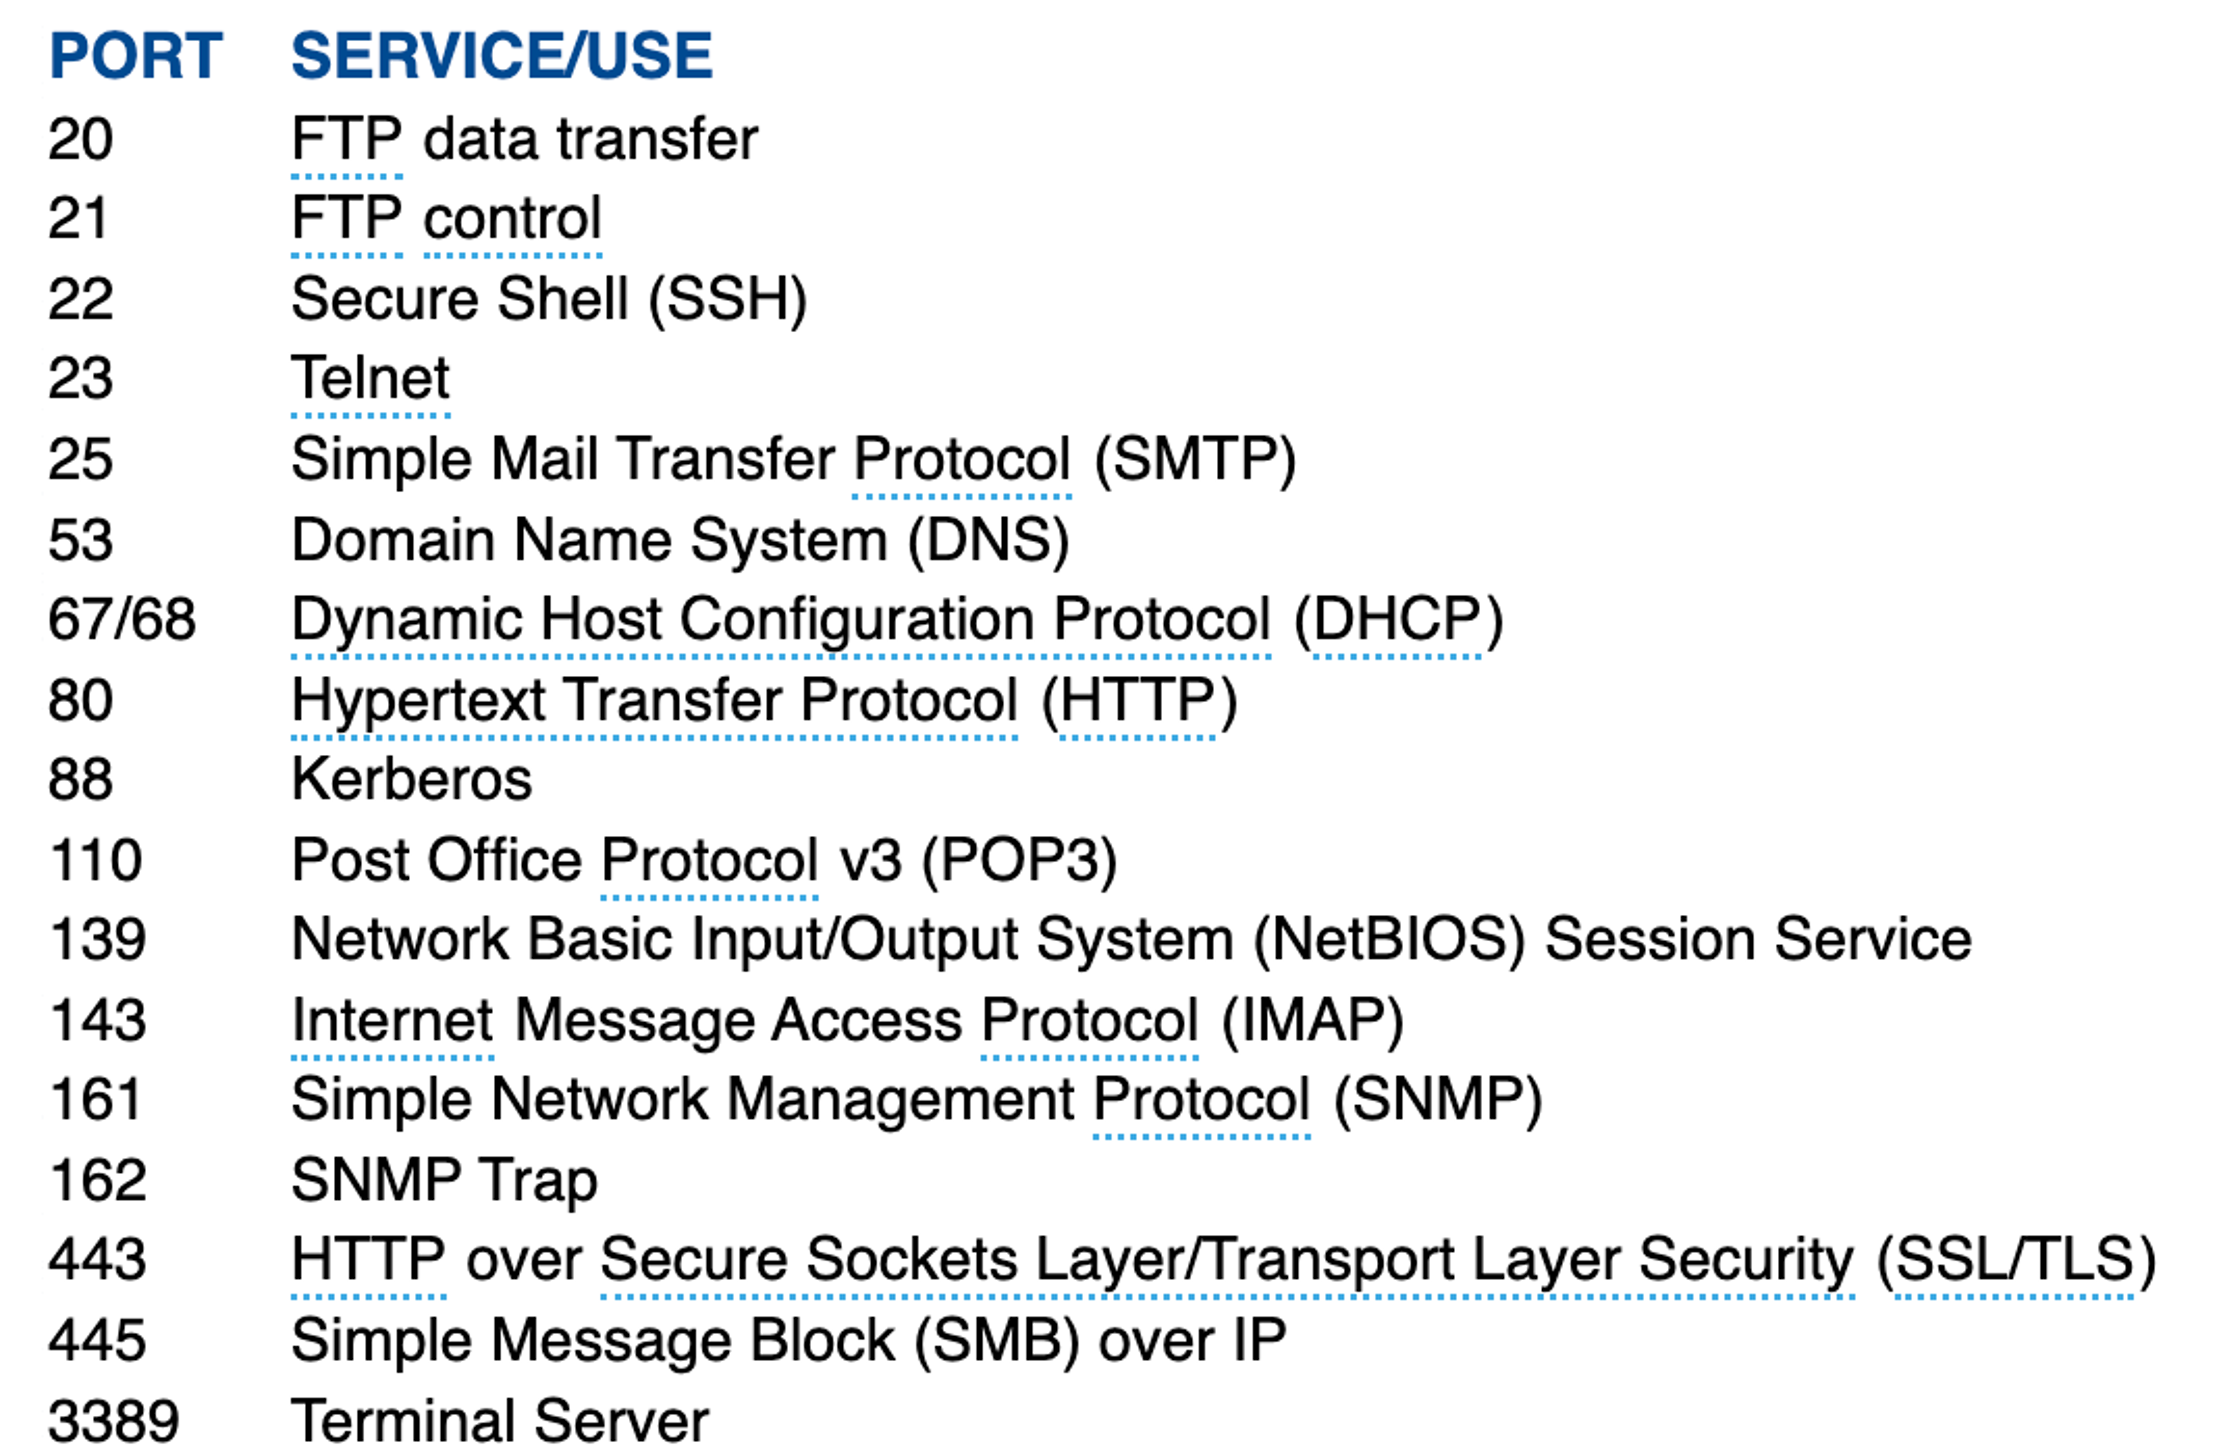
\includegraphics[width=0.8\textwidth]{figuras/image10.png}
            %   \end{center}
            %   
            %   \begin{block}<1->{Puertos Comunes y sus Servicios}
            %   \begin{itemize}
            %   \item<1-> \textbf{Puerto 80}: HTTP (navegación web)
            %   \item<2-> \textbf{Puerto 443}: HTTPS (web seguro)
            %   \item<3-> \textbf{Puerto 22}: SSH (acceso remoto seguro)
            %   \item<4-> \textbf{Puerto 25}: SMTP (envío de correo)
            %   \item<5-> \textbf{Puerto 53}: DNS (resolución de nombres)
            %   \end{itemize}
            %   \end{block}
            %   
            %   \begin{block}<6->{Importancia para la Seguridad}
            %   \begin{itemize}
            %   \item<7-> \textbf{Análisis de tráfico}: Identificar servicios activos
            %   \item<8-> \textbf{Configuración de firewalls}: Bloquear puertos innecesarios
            %   \item<9-> \textbf{Monitoreo de red}: Detectar servicios no autorizados
            %   \item<10-> \textbf{Evaluación de vulnerabilidades}: Identificar puntos de entrada
            %   \end{itemize}
            %   \end{block}
            %   \end{frame}
            %   
            %   % ========================================
            %   % SLIDE 18: Más Detalles de Protocolos
            %   % ========================================
            %   \begin{frame}
            %   \frametitle{Protocolos de Capas Superiores}
            %   
            %   \begin{center}
            %   \Large \textbf{Protocolos de las capas 5, 6 y 7}
            %   \end{center}
            %   
            %   \begin{columns}
            %   \column{0.5\textwidth}
            %   \begin{block}{Capa de Aplicación (7)}
            %   \begin{itemize}
            %   \item \textbf{HTTP}: Protocolo de transferencia de hipertexto
            %   \item \textbf{FTP}: Protocolo de transferencia de archivos
            %   \item \textbf{DNS}: Sistema de nombres de dominio
            %   \item \textbf{SMTP}: Protocolo de correo electrónico
            %   \end{itemize}
            %   \end{block}
            %   
            %   \begin{block}{Capa de Presentación (6)}
            %   \begin{itemize}
            %   \item \textbf{SSL/TLS}: Seguridad en la comunicación
            %   \item \textbf{JPEG}: Compresión de imágenes
            %   \item \textbf{MPEG}: Compresión de video
            %   \item \textbf{ASCII/UTF-8}: Codificación de caracteres
            %   \end{itemize}
            %   \end{block}
            %   
            %   \column{0.5\textwidth}
            %   \begin{block}{Capa de Sesión (5)}
            %   \begin{itemize}
            %   \item \textbf{RPC}: Llamada a procedimiento remoto
            %   \item \textbf{NetBIOS}: Interfaz de red básica
            %   \item \textbf{SQL}: Gestión de sesiones de base de datos
            %   \item \textbf{LDAP}: Protocolo de directorio ligero
            %   \end{itemize}
            %   \end{block}
            %   
            %   \begin{block}{Capa de Transporte (4)}
            %   \begin{itemize}
            %   \item \textbf{TCP}: Control de transmisión (confiable)
            %   \item \textbf{UDP}: Datogramas de usuario (rápido)
            %   \item \textbf{SCTP}: Protocolo de transmisión de flujo
            %   \end{itemize}
            %   \end{block}
            %   \end{columns}
            %   \end{frame}
            %   
            %   \begin{frame}
            %   \frametitle{Protocolos de Capas Inferiores}
            %   
            %   \begin{center}
            %   \Large \textbf{Protocolos de las capas 1, 2 y 3}
            %   \end{center}
            %   
            %   \begin{columns}
            %   \column{0.5\textwidth}
            %   \begin{block}{Capa de Red (3)}
            %   \begin{itemize}
            %   \item \textbf{IP v4}: Direccionamiento de 32 bits
            %   \item \textbf{IP v6}: Direccionamiento de 128 bits
            %   \item \textbf{ICMP}: Mensajes de control y error
            %   \item \textbf{IGMP}: Gestión de grupos de Internet
            %   \item \textbf{OSPF}: Protocolo de enrutamiento
            %   \end{itemize}
            %   \end{block}
            %   
            %   \begin{block}{Capa de Enlace (2)}
            %   \begin{itemize}
            %   \item \textbf{Ethernet}: Estándar de red local
            %   \item \textbf{ARP}: Resolución de direcciones
            %   \item \textbf{PPP}: Protocolo punto a punto
            %   \item \textbf{HDLC}: Control de enlace de datos
            %   \end{itemize}
            %   \end{block}
            %   
            %   \column{0.5\textwidth}
            %   \begin{block}{Capa Física (1)}
            %   \begin{itemize}
            %   \item \textbf{Cable UTP}: Par trenzado sin blindaje
            %   \item \textbf{Fibra óptica}: Transmisión por luz
            %   \item \textbf{Wi-Fi}: Redes inalámbricas IEEE 802.11
            %   \item \textbf{Bluetooth}: Red personal de corto alcance
            %   \item \textbf{Coaxial}: Cable con conductor central
            %   \end{itemize}
            %   \end{block}
            %   
            %   \begin{block}{Estándares}
            %   \begin{itemize}
            %   \item \textbf{IEEE 802.3}: Ethernet
            %   \item \textbf{IEEE 802.11}: Wi-Fi
            %   \item \textbf{ITU-T}: Telecomunicaciones
            %   \end{itemize}
            %   \end{block}
            %   \end{columns}
            %   \end{frame}
            %   
            %   % ========================================
            %   % SLIDE 19: Conceptos Avanzados de Redes
            %   % ========================================
            %   \begin{frame}
            %   \frametitle{Direccionamiento IP y Enrutamiento}
            %   
            %   \begin{center}
            %   \Large \textbf{Conceptos fundamentales de direccionamiento}
            %   \end{center}
            %   
            %   \begin{columns}
            %   \column{0.5\textwidth}
            %   \begin{block}{Direccionamiento IP}
            %   \begin{itemize}
            %   \item \textbf{Clases A, B, C}: División histórica de redes
            %   \item \textbf{CIDR}: Enrutamiento sin clases
            %   \item \textbf{Subnetting}: División de redes en subredes
            %   \item \textbf{VLSM}: Máscaras de subred de longitud variable
            %   \end{itemize}
            %   \end{block}
            %   
            %   \column{0.5\textwidth}
            %   \begin{block}{Enrutamiento}
            %   \begin{itemize}
            %   \item \textbf{Estático}: Rutas configuradas manualmente
            %   \item \textbf{Dinámico}: Rutas aprendidas automáticamente
            %   \item \textbf{Interior}: Dentro de un sistema autónomo
            %   \item \textbf{Exterior}: Entre sistemas autónomos
            %   \end{itemize}
            %   \end{block}
            %   \end{columns}
            %   
            %   \begin{block}{Ventajas del CIDR}
            %   \begin{itemize}
            %   \item \textbf{Agregación}: Múltiples redes en una sola entrada
            %   \item \textbf{Escalabilidad}: Mejor rendimiento en tablas de rutas
            %   \item \textbf{Flexibilidad}: Máscaras de subred de longitud variable
            %   \item \textbf{Eficiencia}: Menor uso de memoria en routers
            %   \end{itemize}
            %   \end{block}
            %   \end{frame}
            %   
            %   \begin{frame}
            %   \frametitle{Conmutación y Calidad de Servicio}
            %   
            %   \begin{center}
            %   \Large \textbf{Técnicas de transferencia de datos}
            %   \end{center}
            %   
            %   \begin{columns}
            %   \column{0.5\textwidth}
            %   \begin{block}{Conmutación}
            %   \begin{itemize}
            %   \item \textbf{Circuitos}: Conexión dedicada
            %   \item \textbf{Paquetes}: Datos divididos en paquetes
            %   \item \textbf{Celdas}: Paquetes de tamaño fijo (ATM)
            %   \item \textbf{Multiplexación}: Compartir un medio
            %   \end{itemize}
            %   \end{block}
            %   
            %   \column{0.5\textwidth}
            %   \begin{block}{Calidad de Servicio}
            %   \begin{itemize}
            %   \item \textbf{Ancho de banda}: Capacidad de transmisión
            %   \item \textbf{Latencia}: Tiempo de respuesta
            %   \item \textbf{Jitter}: Variación en la latencia
            %   \item \textbf{Pérdida de paquetes}: Datos que no llegan
            %   \end{itemize}
            %   \end{block}
            %   \end{columns}
            %   
            %   \begin{block}{Métricas de QoS}
            %   \begin{itemize}
            %   \item \textbf{Throughput}: Datos transmitidos por segundo
            %   \item \textbf{Disponibilidad}: Tiempo de funcionamiento del servicio
            %   \item \textbf{Confiabilidad}: Capacidad de recuperación ante fallas
            %   \item \textbf{Seguridad}: Protección de datos en tránsito
            %   \end{itemize}
            %   \end{block}
            %   \end{frame}
            %   
            %   % ========================================
            %   % SLIDE 20: Arquitectura de Redes Modernas
            %   % ========================================
            %   \begin{frame}
            %   \frametitle{Topologías y Dispositivos de Red}
            %   
            %   \begin{center}
            %   \Large \textbf{¿Cómo se organizan las redes actuales?}
            %   \end{center}
            %   
            %   \begin{columns}
            %   \column{0.5\textwidth}
            %   \begin{block}{Topologías de Red}
            %   \begin{itemize}
            %   \item \textbf{Estrella}: Todos los nodos conectados a un centro
            %   \item \textbf{Anillo}: Nodos conectados en círculo
            %   \item \textbf{Bus}: Todos los nodos en una línea común
            %   \item \textbf{Malla}: Múltiples conexiones entre nodos
            %   \item \textbf{Árbol}: Estructura jerárquica
            %   \end{itemize}
            %   \end{block}
            %   
            %   \column{0.5\textwidth}
            %   \begin{block}{Dispositivos de Red}
            %   \begin{itemize}
            %   \item \textbf{Hubs}: Repetidores multipuerto (obsoletos)
            %   \item \textbf{Switches}: Conmutadores inteligentes
            %   \item \textbf{Routers}: Enrutadores entre redes
            %   \item \textbf{Access Points}: Puntos de acceso Wi-Fi
            %   \item \textbf{Firewalls}: Control de tráfico
            %   \end{itemize}
            %   \end{block}
            %   \end{columns}
            %   
            %   \begin{block}{Selección de Topología}
            %   \begin{itemize}
            %   \item \textbf{Costo}: Presupuesto disponible para implementación
            %   \item \textbf{Escalabilidad}: Capacidad de crecimiento futuro
            %   \item \textbf{Confiabilidad}: Tolerancia a fallas
            %   \item \textbf{Mantenimiento}: Facilidad de administración
            %   \end{itemize}
            %   \end{block}
            %   \end{frame}
            %   
            %   \begin{frame}
            %   \frametitle{Medios de Transmisión y Características}
            %   
            %   \begin{center}
            %   \Large \textbf{¿Cómo se transmiten los datos físicamente?}
            %   \end{center}
            %   
            %   \begin{block}{Medios de Transmisión}
            %   \begin{itemize}
            %   \item \textbf{Guía}: Cable, fibra (dirección fija)
            %   \item \textbf{No guía}: Radio, microondas, satélite
            %   \item \textbf{Simplex}: Una dirección
            %   \item \textbf{Duplex}: Dos direcciones
            %   \item \textbf{Full-duplex}: Ambas direcciones simultáneas
            %   \end{itemize}
            %   \end{block}
            %   
            %   \begin{columns}
            %   \column{0.5\textwidth}
            %   \begin{block}{Ventajas de Medios Guiados}
            %   \begin{itemize}
            %   \item \textbf{Seguridad}: Difícil interceptar sin acceso físico
            %   \item \textbf{Rendimiento}: Menor interferencia y pérdida
            %   \item \textbf{Confiabilidad}: Menos afectado por condiciones ambientales
            %   \item \textbf{Ancho de banda}: Mayor capacidad de transmisión
            %   \end{itemize}
            %   \end{block}
            %   
            %   \column{0.5\textwidth}
            %   \begin{block}{Ventajas de Medios No Guiados}
            %   \begin{itemize}
            %   \item \textbf{Movilidad}: No requiere conexión física
            %   \item \textbf{Instalación}: Más fácil de implementar
            %   \item \textbf{Cobertura}: Puede alcanzar áreas remotas
            %   \item \textbf{Flexibilidad}: Fácil reconfiguración
            %   \end{itemize}
            %   \end{block}
            %   \end{columns}
            %   \end{frame}
            %   
            %   % ========================================
            %   % SLIDE: Topologías de Red Visual
            %   % ========================================
            %   \begin{frame}
            %   \frametitle{Topologías de Red - Representación Visual}
            %   
            %   \begin{center}
            %   \Large \textbf{Diferentes formas de conectar dispositivos}
            %   \end{center}
            %   
            %   \begin{center}
            %   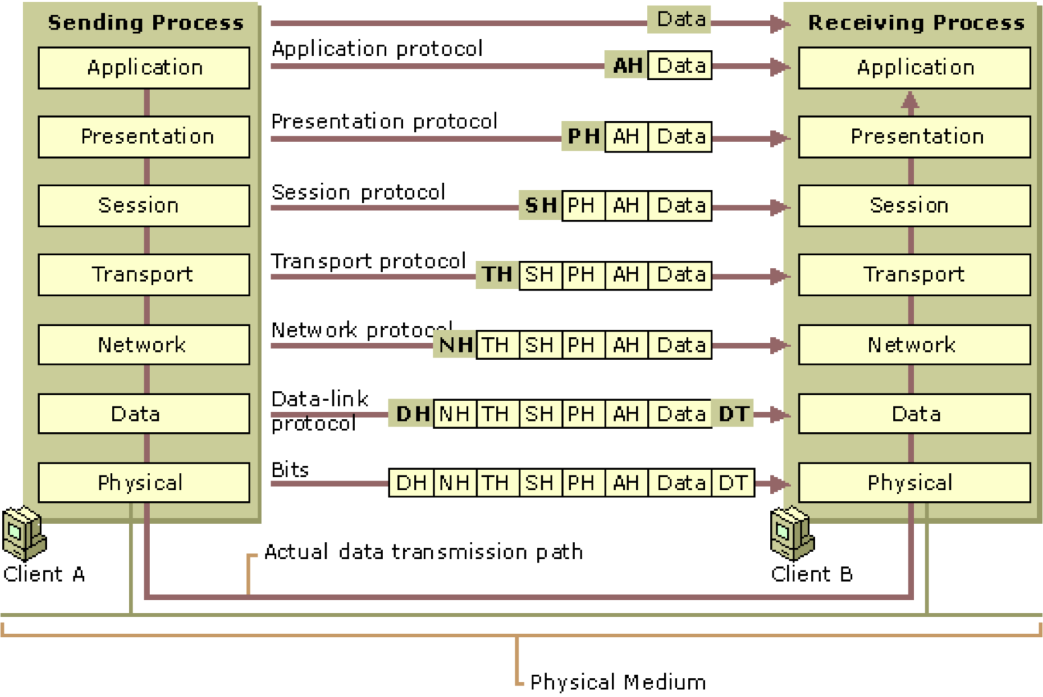
\includegraphics[width=0.85\textwidth]{figuras/image9.png}
            %   \end{center}
            %   
            %   \begin{block}{Ventajas y Desventajas}
            %   \begin{itemize}
            %   \item \textbf{Estrella}: Fácil mantenimiento, punto único de falla
            %   \item \textbf{Anillo}: Eficiente, pero si se rompe un enlace se pierde la red
            %   \item \textbf{Malla}: Muy confiable, pero costosa de implementar
            %   \item \textbf{Árbol}: Escalable, pero dependiente del nodo raíz
            %   \end{itemize}
            %   \end{block}
            %   \end{frame}
            %   
            %   % ========================================
            %   % SLIDE 21: Calidad de Servicio y Rendimiento
            %   % ========================================
            %   \begin{frame}
            %   \frametitle{Métricas de Rendimiento de Red}
            %   
            %   \begin{center}
            %   \Large \textbf{¿Cómo medimos el rendimiento de una red?}
            %   \end{center}
            %   
            %   \begin{block}{Métricas de Rendimiento}
            %   \begin{itemize}
            %   \item \textbf{Ancho de banda}: Capacidad de transmisión (bits/segundo)
            %   \item \textbf{Throughput}: Datos reales transmitidos por segundo
            %   \item \textbf{Latencia}: Tiempo de ida y vuelta (RTT)
            %   \item \textbf{Jitter}: Variación en la latencia
            %   \item \textbf{Pérdida de paquetes}: Porcentaje de datos perdidos
            %   \end{itemize}
            %   \end{block}
            %   
            %   \begin{block}{Importancia de las Métricas}
            %   \begin{itemize}
            %   \item \textbf{Diagnóstico}: Identificar problemas de rendimiento
            %   \item \textbf{Planificación}: Dimensionar recursos adecuadamente
            %   \item \textbf{Monitoreo}: Seguimiento continuo del servicio
            %   \item \textbf{Optimización}: Mejorar la experiencia del usuario
            %   \end{itemize}
            %   \end{block}
            %   \end{frame}
            %   
            %   \begin{frame}
            %   \frametitle{Factores y Herramientas de Medición}
            %   
            %   \begin{center}
            %   \Large \textbf{¿Qué afecta el rendimiento y cómo medirlo?}
            %   \end{center}
            %   
            %   \begin{columns}
            %   \column{0.5\textwidth}
            %   \begin{block}{Factores que Afectan el Rendimiento}
            %   \begin{itemize}
            %   \item \textbf{Distancia}: Cuanto más lejos, más latencia
            %   \item \textbf{Medio físico}: Fibra vs cable vs Wi-Fi
            %   \item \textbf{Congestión}: Muchos usuarios simultáneos
            %   \item \textbf{Interferencias}: Señales que se interfieren
            %   \item \textbf{Calidad del hardware}: Dispositivos antiguos
            %   \end{itemize}
            %   \end{block}
            %   
            %   \column{0.5\textwidth}
            %   \begin{block}{Herramientas de Medición}
            %   \begin{itemize}
            %   \item \textbf{Ping}: Medir latencia básica
            %   \item \textbf{Traceroute}: Ruta de los paquetes
            %   \item \textbf{Speedtest}: Medir ancho de banda
            %   \item \textbf{Wireshark}: Analizar tráfico de red
            %   \item \textbf{Netstat}: Estadísticas de conexiones
            %   \end{itemize}
            %   \end{block}
            %   \end{columns}
            %   
            %   \begin{block}{Mejores Prácticas de Medición}
            %   \begin{itemize}
            %   \item \textbf{Consistencia}: Medir en los mismos horarios
            %   \item \textbf{Documentación}: Registrar condiciones de la medición
            %   \item \textbf{Análisis}: Comparar resultados a lo largo del tiempo
            %   \item \textbf{Acción}: Tomar medidas basadas en los datos
            %   \end{itemize}
            %   \end{block}
            %   \end{frame}
            %   
            %   % ========================================
            %   % SLIDE: Métricas de Red Visual
            %   % ========================================
            %   \begin{frame}
            %   \frametitle{Métricas de Red - Representación Visual}
            %   
            %   \begin{center}
            %   \Large \textbf{Medición y monitoreo del rendimiento}
            %   \end{center}
            %   
            %   \begin{center}
            %   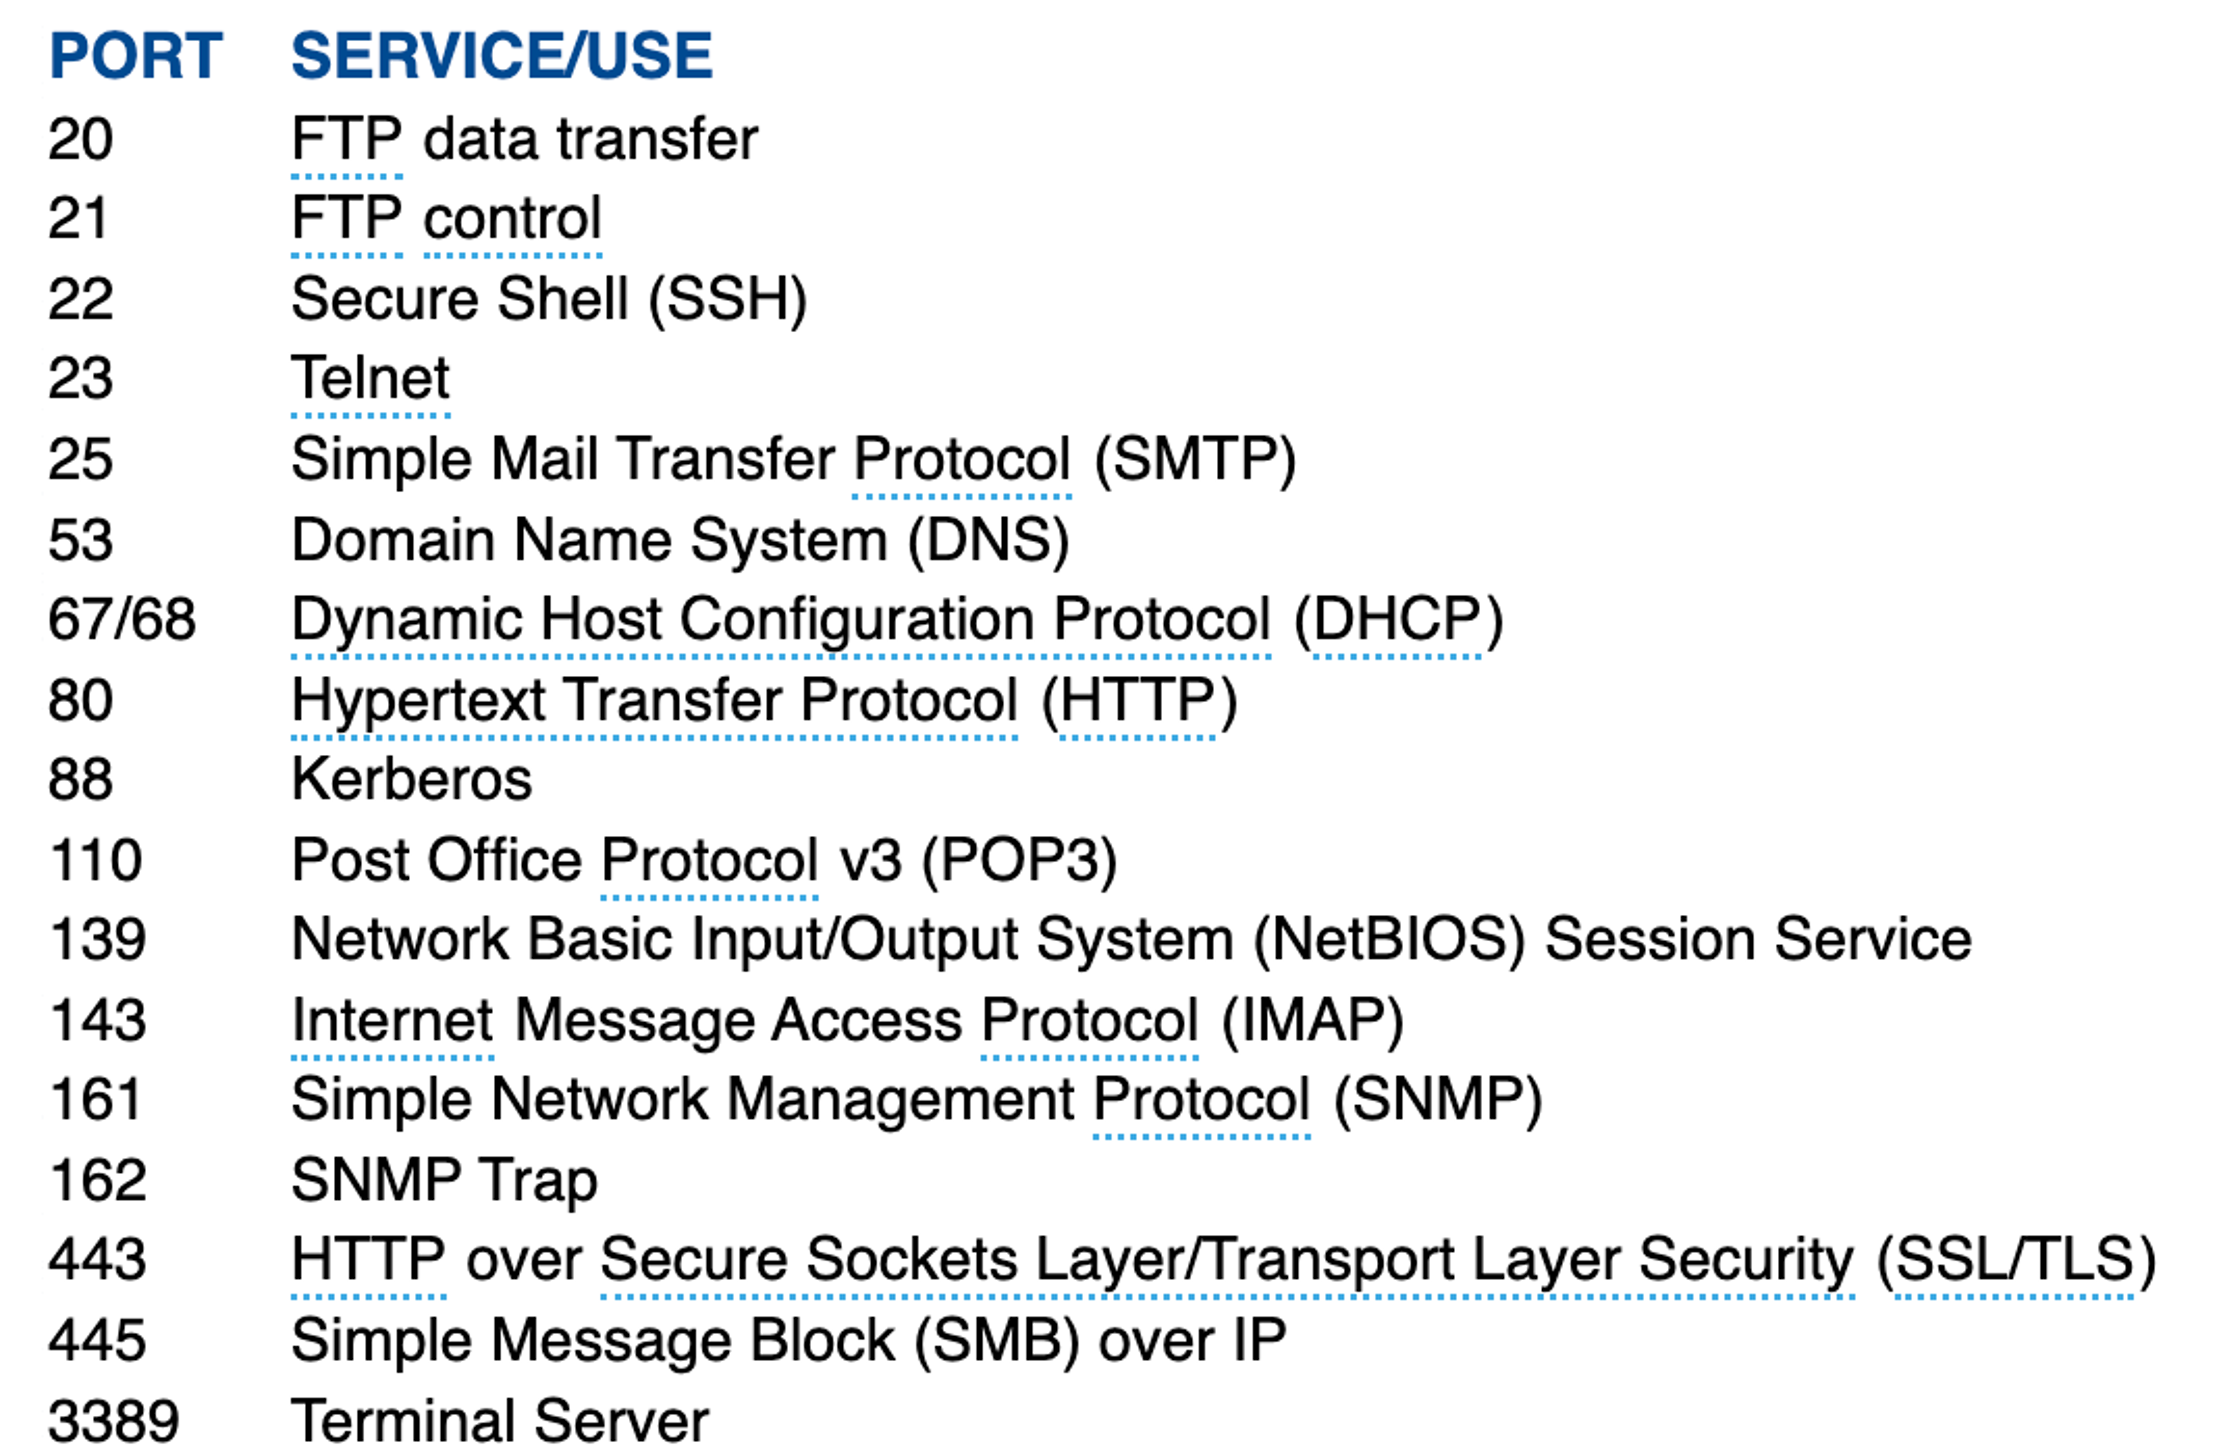
\includegraphics[width=0.85\textwidth]{figuras/image10.png}
            %   \end{center}
            %   
            %   \begin{block}{Herramientas de Monitoreo}
            %   \begin{itemize}
            %   \item \textbf{Monitoreo en tiempo real}: Ping, traceroute, netstat
            %   \item \textbf{Análisis de tráfico}: Wireshark, tcpdump
            %   \item \textbf{Monitoreo de ancho de banda}: Speedtest, iperf
            %   \item \textbf{Monitoreo de dispositivos}: SNMP, Nagios
            %   \end{itemize}
            %   \end{block}
            %   \end{frame}
            %   
            %   % ========================================
            %   % SLIDE: Análisis de Paquetes
            %   % ========================================
            %   \begin{frame}
            %   \frametitle{Visualización de Paquetes de Red}
            %   
            %   \begin{center}
            %   \Large \textbf{¿Cómo se ve un paquete real en la red?}
            %   \end{center}
            %   
            %   \begin{center}
            %   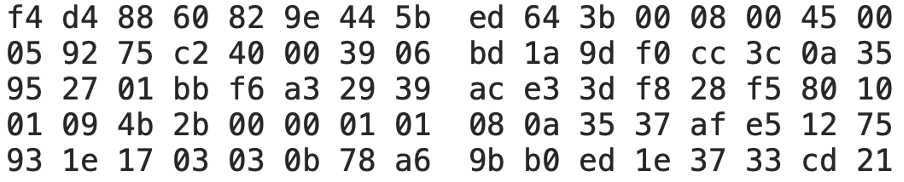
\includegraphics[width=0.8\textwidth]{figuras/image11.png}
            %   \end{center}
            %   
            %   \begin{block}{¿Qué nos muestra esta imagen?}
            %   \begin{itemize}
            %   \item \textbf{Hex dump}: Representación hexadecimal del paquete
            %   \item \textbf{Análisis visual}: Estructura organizada por bytes
            %   \item \textbf{Información de red}: Encabezados de protocolos
            %   \item \textbf{Datos de aplicación}: Contenido real transmitido
            %   \end{itemize}
            %   \end{block}
            %   \end{frame}
            %   
            %   \begin{frame}
            %   \frametitle{Análisis e Interpretación de Paquetes}
            %   
            %   \begin{center}
            %   \Large \textbf{¿Cómo extraer información útil del hex dump?}
            %   \end{center}
            %   
            %   \begin{columns}
            %   \column{0.5\textwidth}
            %   \begin{block}{Extracción de Información del Hex Dump}
            %   \begin{itemize}
            %   \item \textbf{Dirección IP de Origen}: 9d f0 cc 3c (157.240.204.60)
            %   \item \textbf{Dirección IP de Destino}: 0a 35 95 27 (10.53.149.39)
            %   \item \textbf{Puerto de Origen}: 01 bb (443 en decimal)
            %   \item \textbf{Puerto de Destino}: f6 a3 (63139 en decimal)
            %   \item \textbf{Protocolo}: 06 (TCP)
            %   \end{itemize}
            %   \end{block}
            %   
            %   \column{0.5\textwidth}
            %   \begin{block}{Herramientas de Análisis}
            %   \begin{itemize}
            %   \item \textbf{Wireshark}: Analizador de protocolos gráfico
            %   \item \textbf{tcpdump}: Captura de paquetes en línea de comandos
            %   \item \textbf{Análisis hexadecimal}: Interpretación manual de datos
            %   \item \textbf{Identificación de patrones}: Detección de malware y anomalías
            %   \end{itemize}
            %   \end{block}
            %   \end{columns}
            %   
            %   \begin{block}{Aplicaciones del Análisis de Paquetes}
            %   \begin{itemize}
            %   \item \textbf{Seguridad}: Detectar tráfico malicioso
            %   \item \textbf{Depuración}: Resolver problemas de conectividad
            %   \item \textbf{Optimización}: Mejorar rendimiento de aplicaciones
            %   \item \textbf{Monitoreo}: Supervisar uso de la red
            %   \end{itemize}
            %   \end{block}
            %   \end{frame}
            %   
            %   % ========================================
            %   % SLIDE 22: Lectura Recomendada
            %   % ========================================
            %   \begin{frame}
            %   \frametitle{Lectura Recomendada}
            %   
            %   \begin{center}
            %   \Large \textbf{Continúa tu aprendizaje}
            %   \end{center}
            %   
            %   \begin{block}{Libro Principal}
            %   \textbf{Andrew S. Tanenbaum – Computer Networks}
            %   \begin{itemize}
            %   \item \textbf{Capítulo 1}: Introducción a redes
            %   \item \textbf{Capítulo 2}: Modelo OSI y arquitectura de red
            %   \item \textbf{Capítulo 3}: Protocolos TCP/IP
            %   \item \textbf{Capítulo 4}: Capas de red y transporte
            %   \end{itemize}
            %   \end{block}
            %   
            %   \begin{block}{Recursos Adicionales}
            %   \begin{itemize}
            %   \item \textbf{Online}: Cisco Networking Academy
            %   \item \textbf{Videos}: YouTube - "Modelo OSI explicado"
            %   \item \textbf{Práctica}: Packet Tracer, Wireshark
            %   \end{itemize}
            %   \end{block}
            %   
            %   \begin{block}{Próximo Paso}
            %   \textbf{En la siguiente sesión}: Aplicaremos estos conceptos a la seguridad de redes
            %   \end{block}
            %   \end{frame}
              
              % ========================================
              % SLIDE FINAL: Resumen
              % ========================================
              \begin{frame}
              \frametitle{Resumen de la Sesión}
              
              \begin{center}
              \Large \textbf{¿Qué hemos aprendido hoy?}
              \end{center}
              
              \begin{columns}
              \column{0.5\textwidth}
              \begin{block}{Conceptos Clave}
              \begin{itemize}
              \item \textbf{Redes}: Sistemas de comunicación entre dispositivos
              \item \textbf{Evolución}: De telégrafos a Internet
              \item \textbf{Paquetes}: Unidades básicas de datos en la red
              \item \textbf{Packet Switching}: Mejor que circuit switching para datos
              \item \textbf{Modelo OSI}: Arquitectura de 7 capas
              \end{itemize}
              \end{block}
              
              \column{0.5\textwidth}
              \begin{block}{Analogías Utilizadas}
              \begin{itemize}
              \item \textbf{Edificio}: 7 pisos con funciones específicas
              \item \textbf{Ciudad}: Calles, direcciones y servicios
              \item \textbf{Mensajería}: Envío de paquetes de datos
              \item \textbf{Traductor}: Conversión de formatos
              \end{itemize}
              \end{block}
              \end{columns}
  
              \begin{center}
              \Large \textbf{¡Gracias por tu atención!}
              \end{center}
              \end{frame}
      
\end{document}
